\section*{Appendix A} \label{A}

Az ábrákon szereplő adatok sorrendben a követkeezőek:
\begin{enumerate}
    \item A pillanatnyi mért hőméréskéletek a teljes futtatás során: (\ref{fig:1}) és (\ref{fig:13})
    \item A pillanatnyi mért hőméréskéletek az egyensúy beállta utén (\ref{fig:2}) és (\ref{fig:14})
    \item A rendszer teljes energiája a futtatás egésze során: (\ref{fig:3}) és (\ref{fig:15})
    \item A teljes energia az egyensúlyi helyzet után: (\ref{fig:4}) és (\ref{fig:16})
    \item A rendszerben mérhető $\sum_{i < j} \boldsymbol{r}_{ij} \boldsymbol{F}_{ij}$ munkák: (\ref{fig:5}) és (\ref{fig:17})
    \item Ugyanezen munkák az egyensúlyi állapotban: (\ref{fig:6}) és (\ref{fig:18})
    \item Az energia időátlagának fejlődése az egyensúlyi állapot után: (\ref{fig:7}) és (\ref{fig:19})
    \item Az energianégyzet időátlagának fejlődése: (\ref{fig:8}) és (\ref{fig:20})
    \item Az energia szórásnégyzete az egyensúlyi állapot után: (\ref{fig:9}) és (\ref{fig:21})
    \item Az egyensúly beállta után mért moláris hőkapacitás $C_{V}$: (\ref{fig:10}) és (\ref{fig:22})
    \item A $PV$ függvény ábrázolása: (\ref{fig:11}) és (\ref{fig:23})
    \item A kompresszibilitási faktor ($Z$): (\ref{fig:12}) és (\ref{fig:24})
\end{enumerate}
A mennyiségekről készült ábrák a következő oldalon kezdődnek!

\newpage

\subsection*{A.1.1\ \ Mérendő mennyiségek adatai $n=12000$ lépés esetén} \label{A.1.1}

{\centering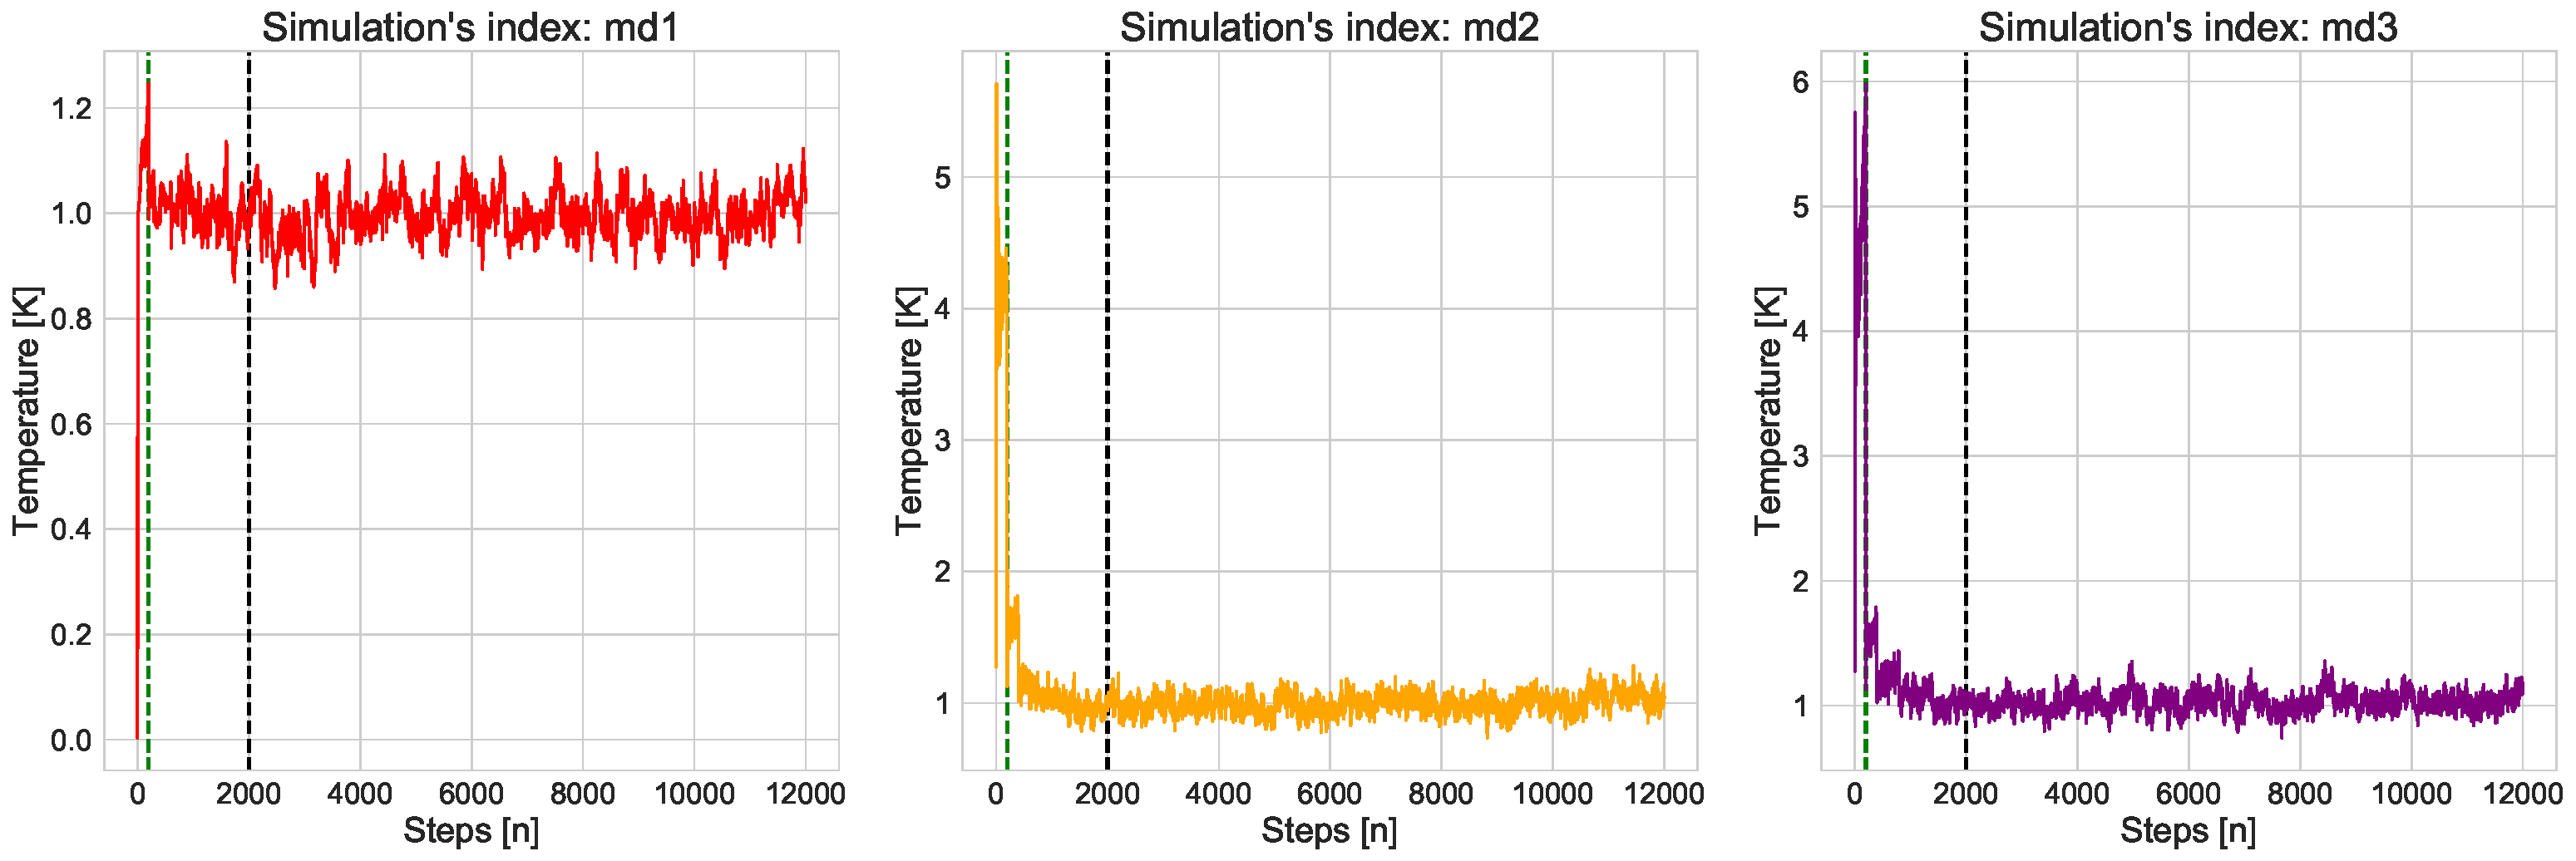
\includegraphics[width=\textwidth]{images/instantaneous_temperatures_12.pdf}}
\captionof{figure}{Pillanatnyi hőmérsékletek zárt rendszerben, $N = 64$ részecske esetén} \label{fig:1}
\hfill \break \break
{\centering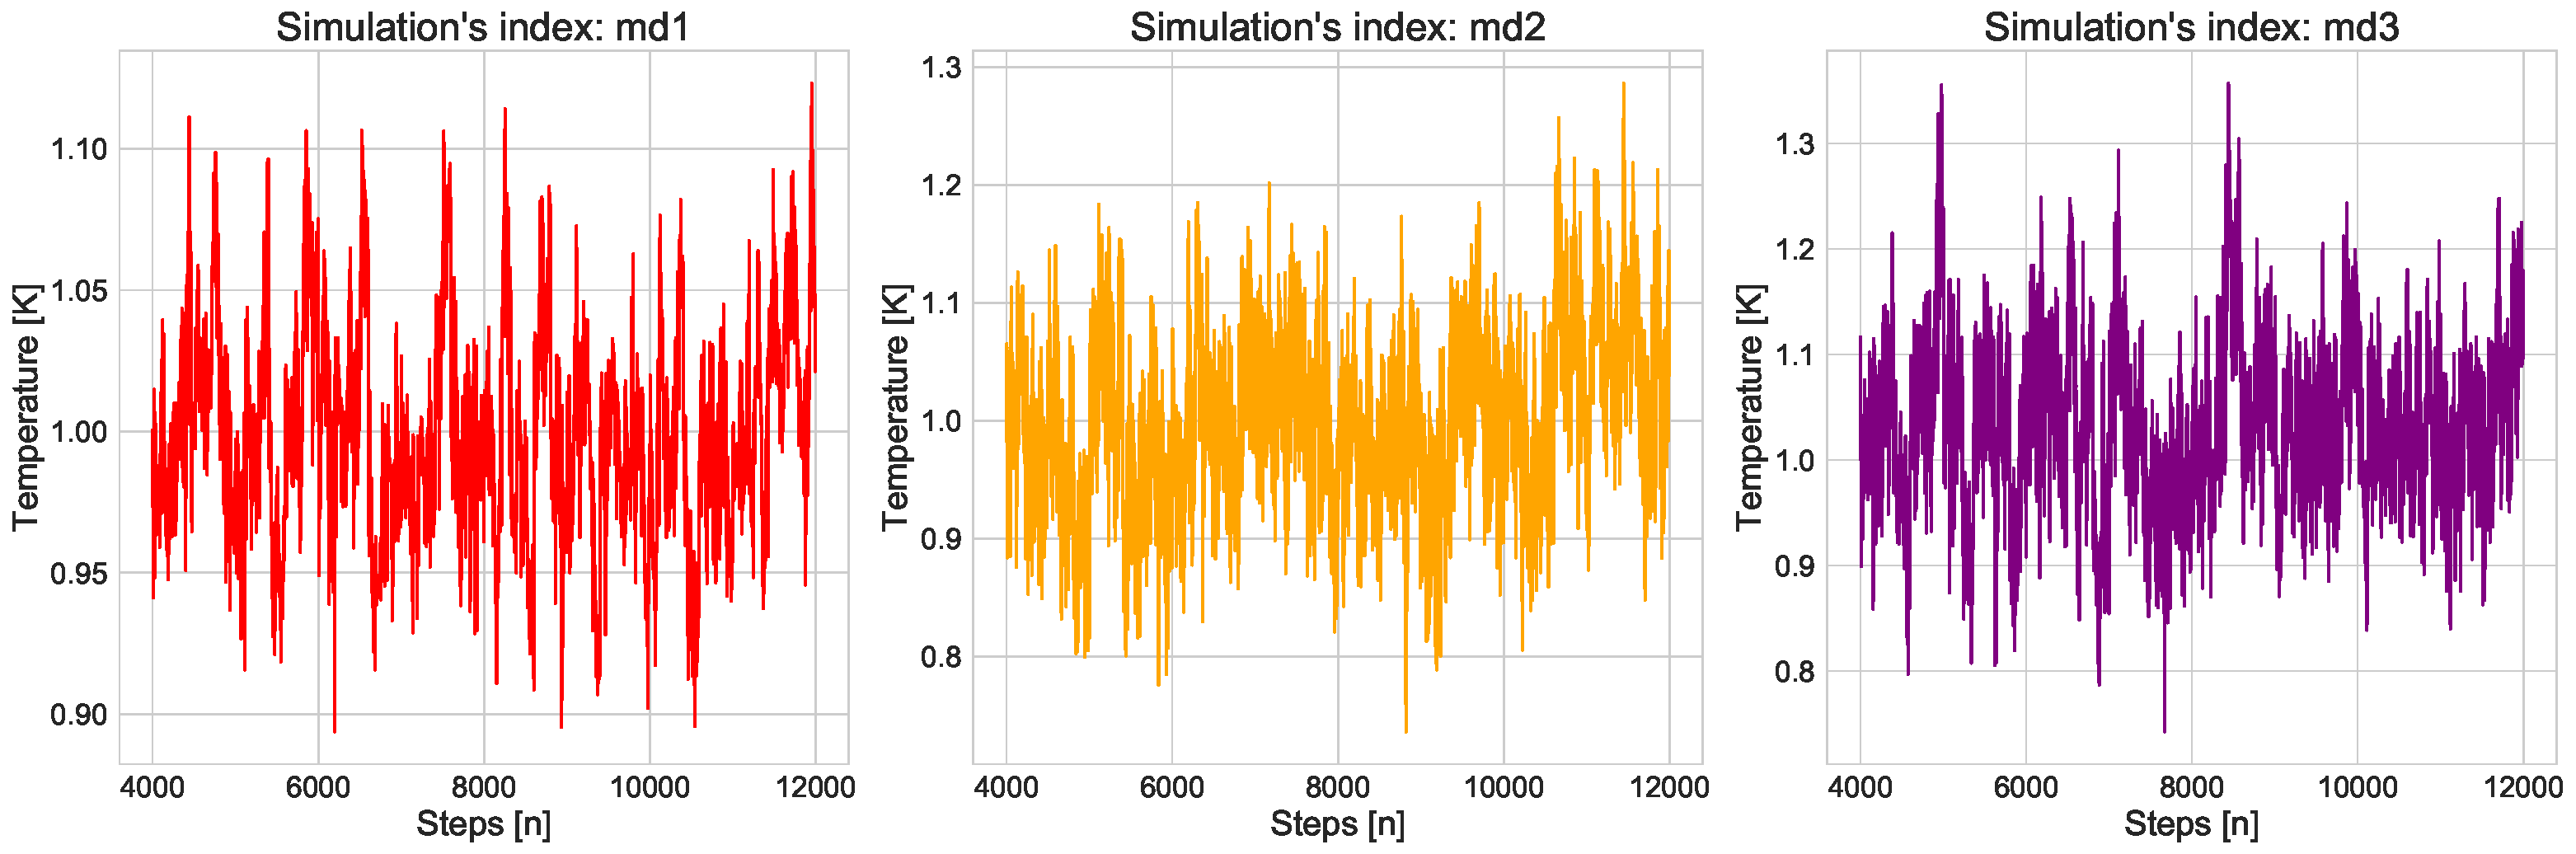
\includegraphics[width=\textwidth]{images/instantaneous_temperatures_equi_12.pdf}}
\captionof{figure}{Pillanatnyi hőmérsékletek zárt rendszerben, az egyensúlyi állapotban, $N = 64$ részecske esetén} \label{fig:2}
\hfill \break \break
{\centering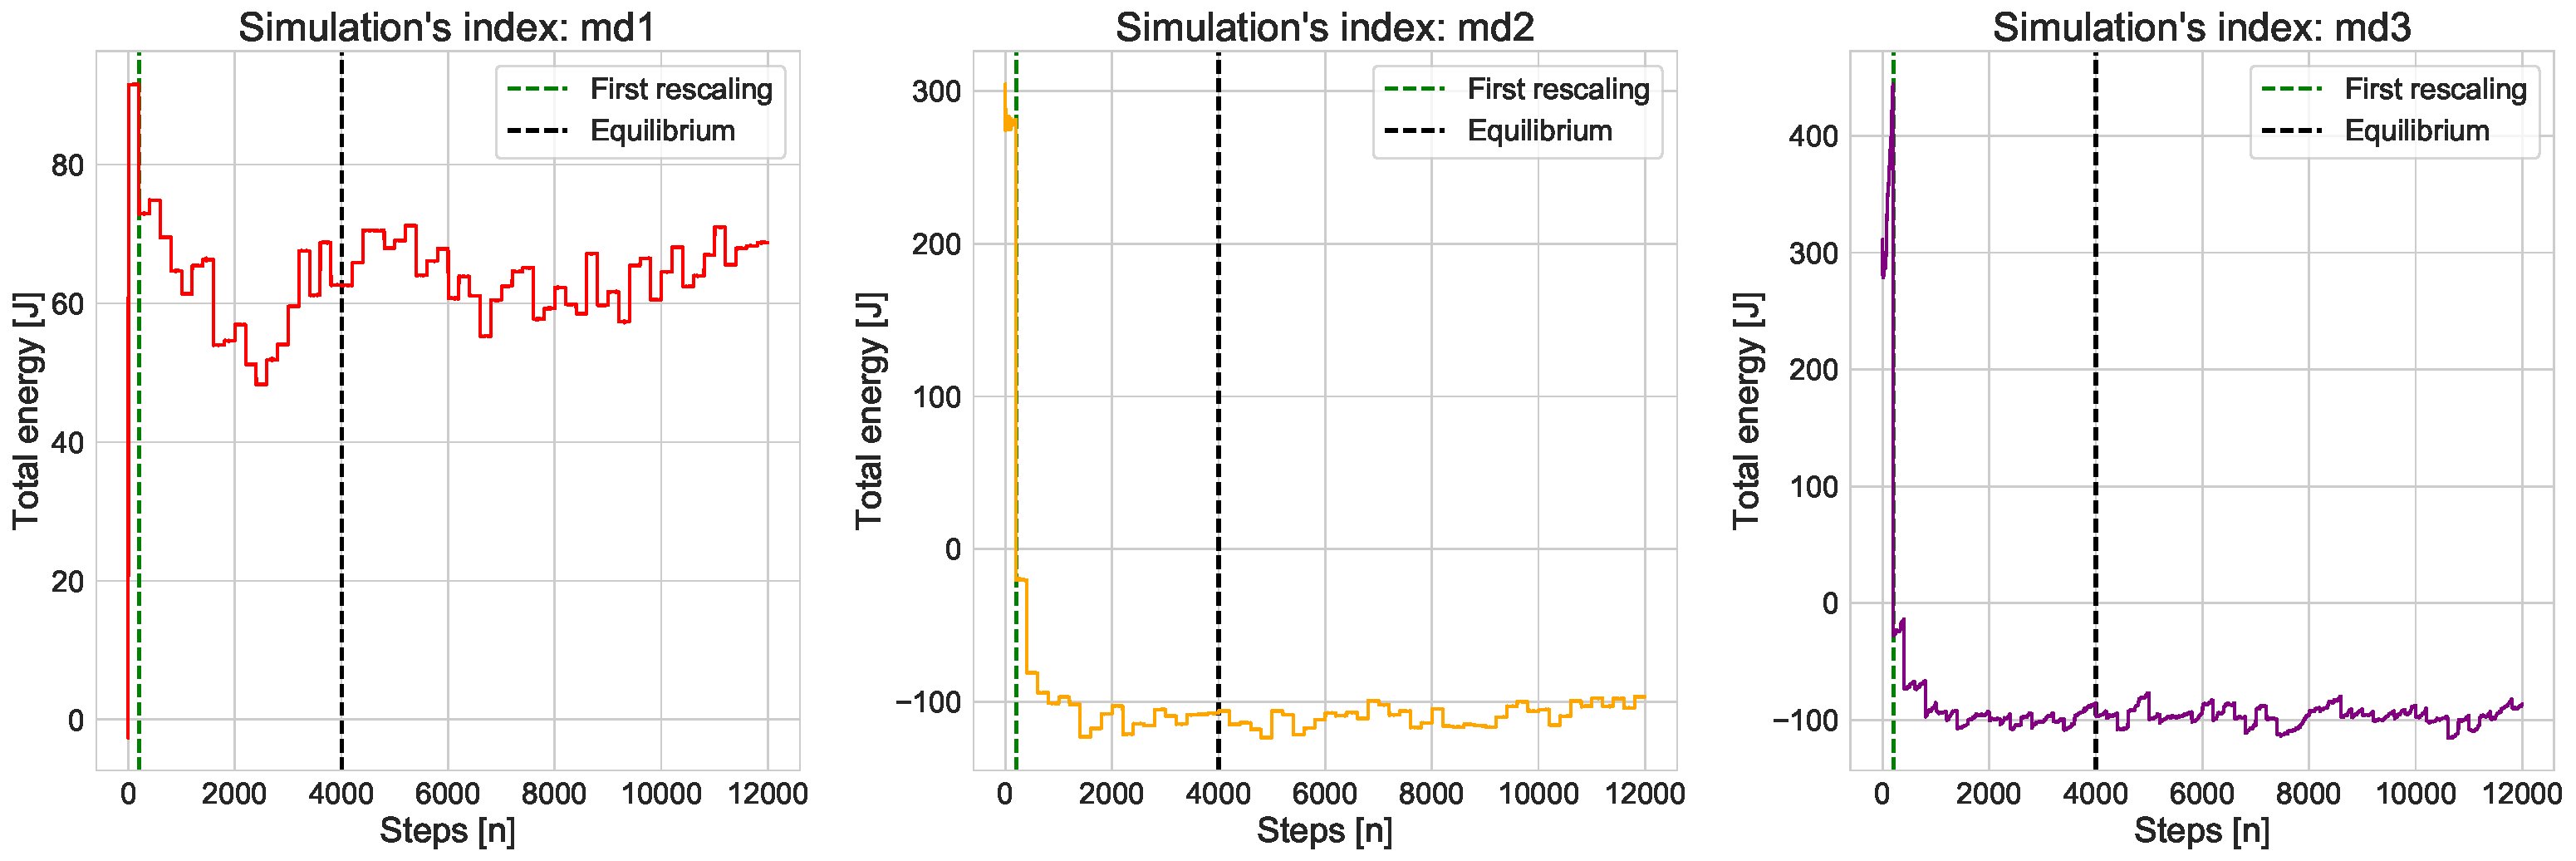
\includegraphics[width=\textwidth]{images/total_energy_12.pdf}}
\captionof{figure}{A zárt rendszer teljes energiája $N = 64$ részecske esetén} \label{fig:3}
\hfill \break \break
{\centering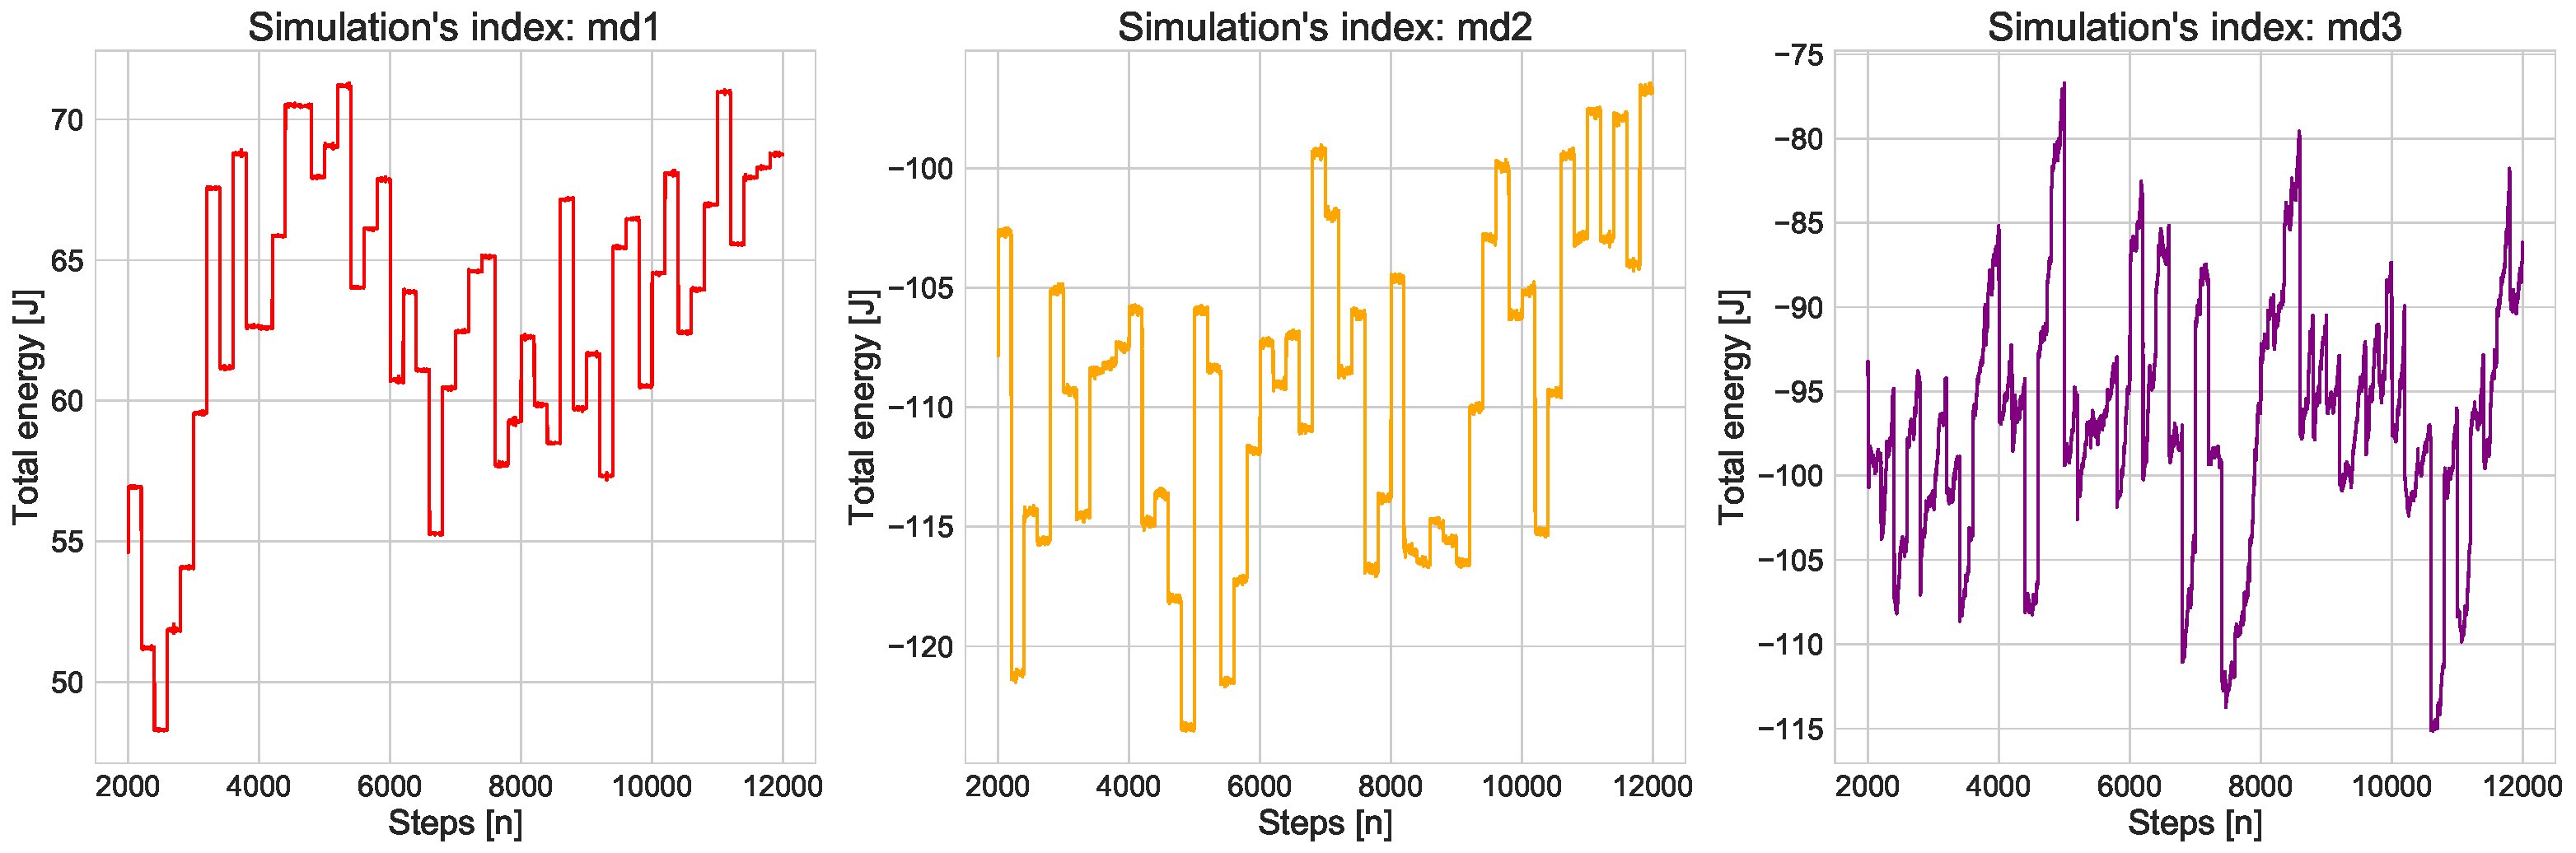
\includegraphics[width=\textwidth]{images/total_energy_equi_12.pdf}}
\captionof{figure}{A zárt rendszer teljes energiája az egyensúlyi állapotban $N = 64$ részecske esetén} \label{fig:4}

\newpage

{\centering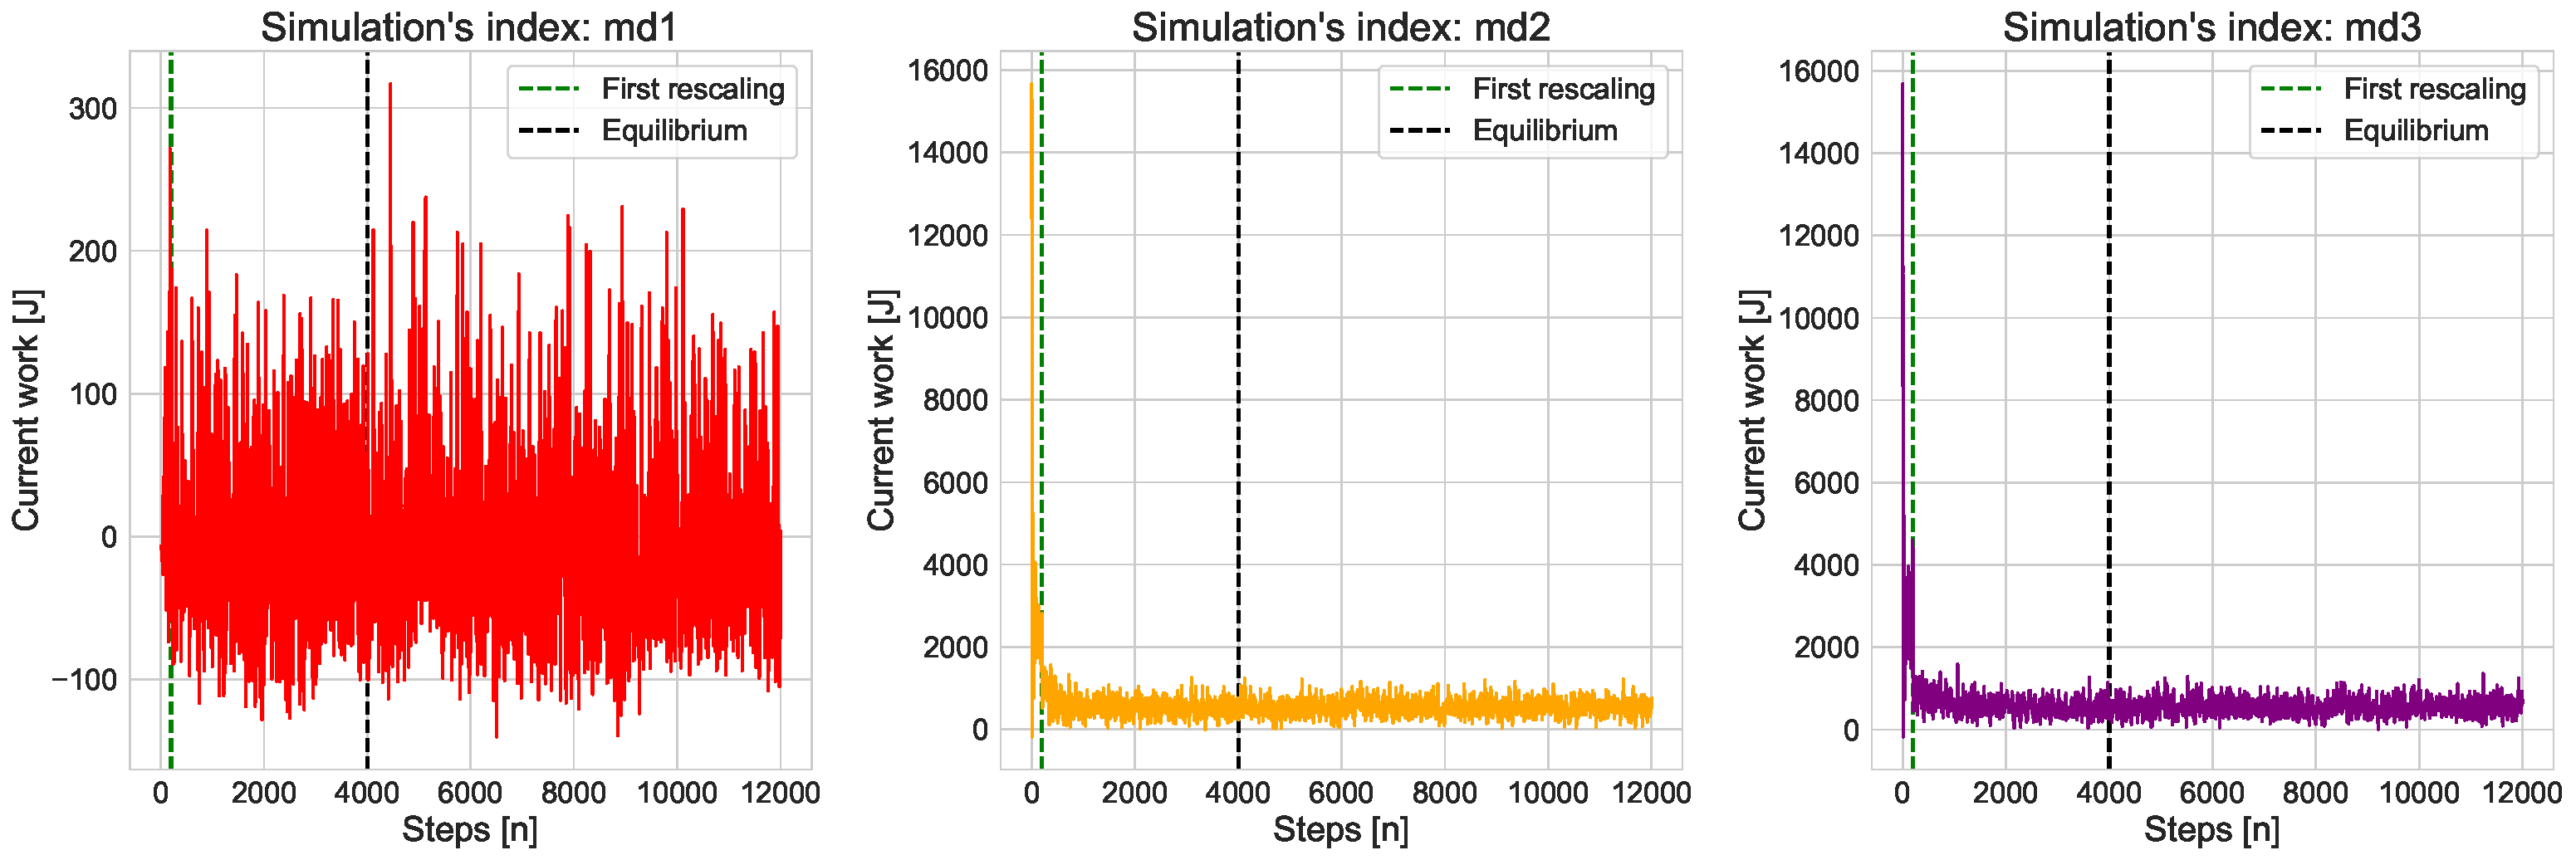
\includegraphics[width=\textwidth]{images/virial_12.pdf}}
\captionof{figure}{A mérhető munka időátlaga ($\left< \sum_{i < j} \boldsymbol{r}_{ij} \cdot \boldsymbol{F}_{ij} \right>$) $N = 64$ részecske esetén} \label{fig:5}
\hfill \break \break
{\centering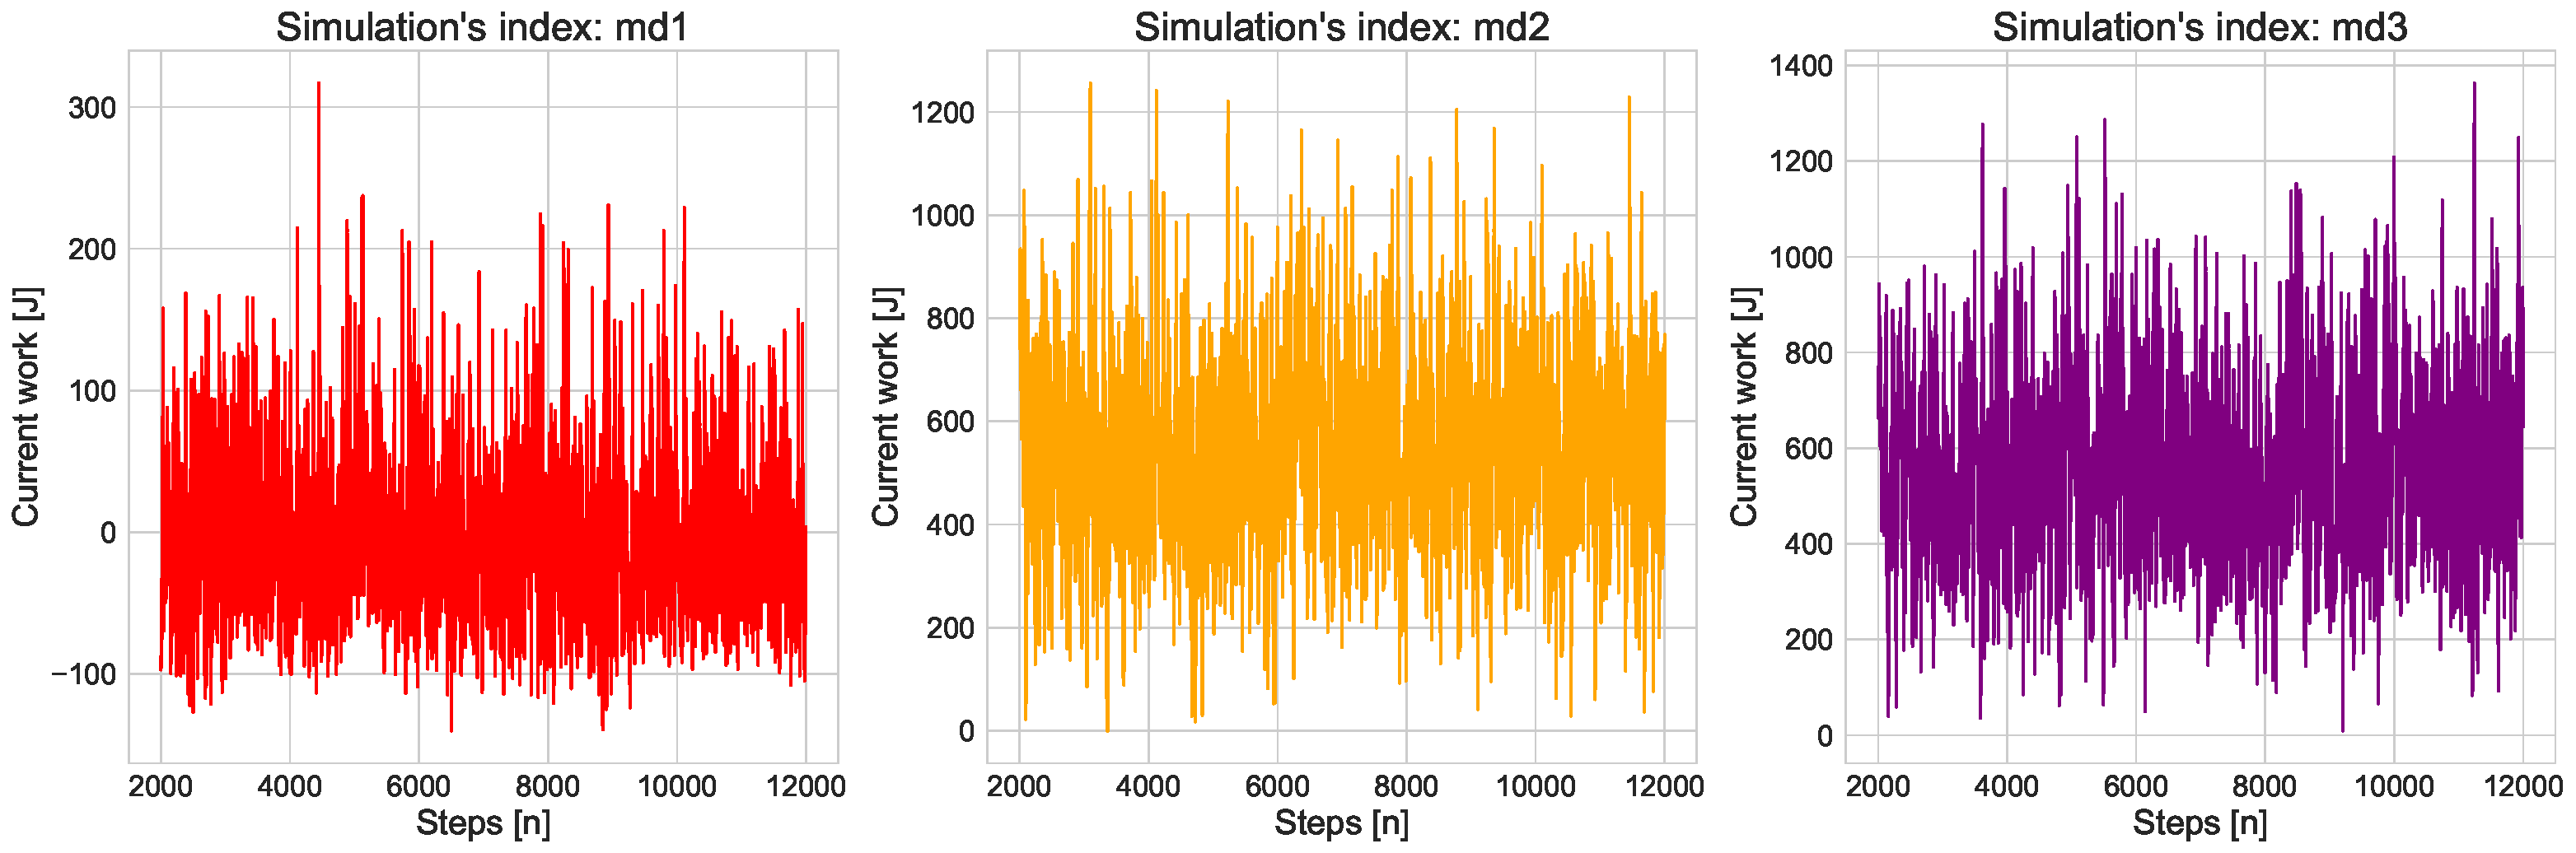
\includegraphics[width=\textwidth]{images/virial_equi_12.pdf}}
\captionof{figure}{A mérhető munka időátlaga az egyensúlyi állapotban ($\left< \sum_{i < j} \boldsymbol{r}_{ij} \cdot \boldsymbol{F}_{ij} \right>$) $N = 64$ részecske esetén} \label{fig:6}
{\centering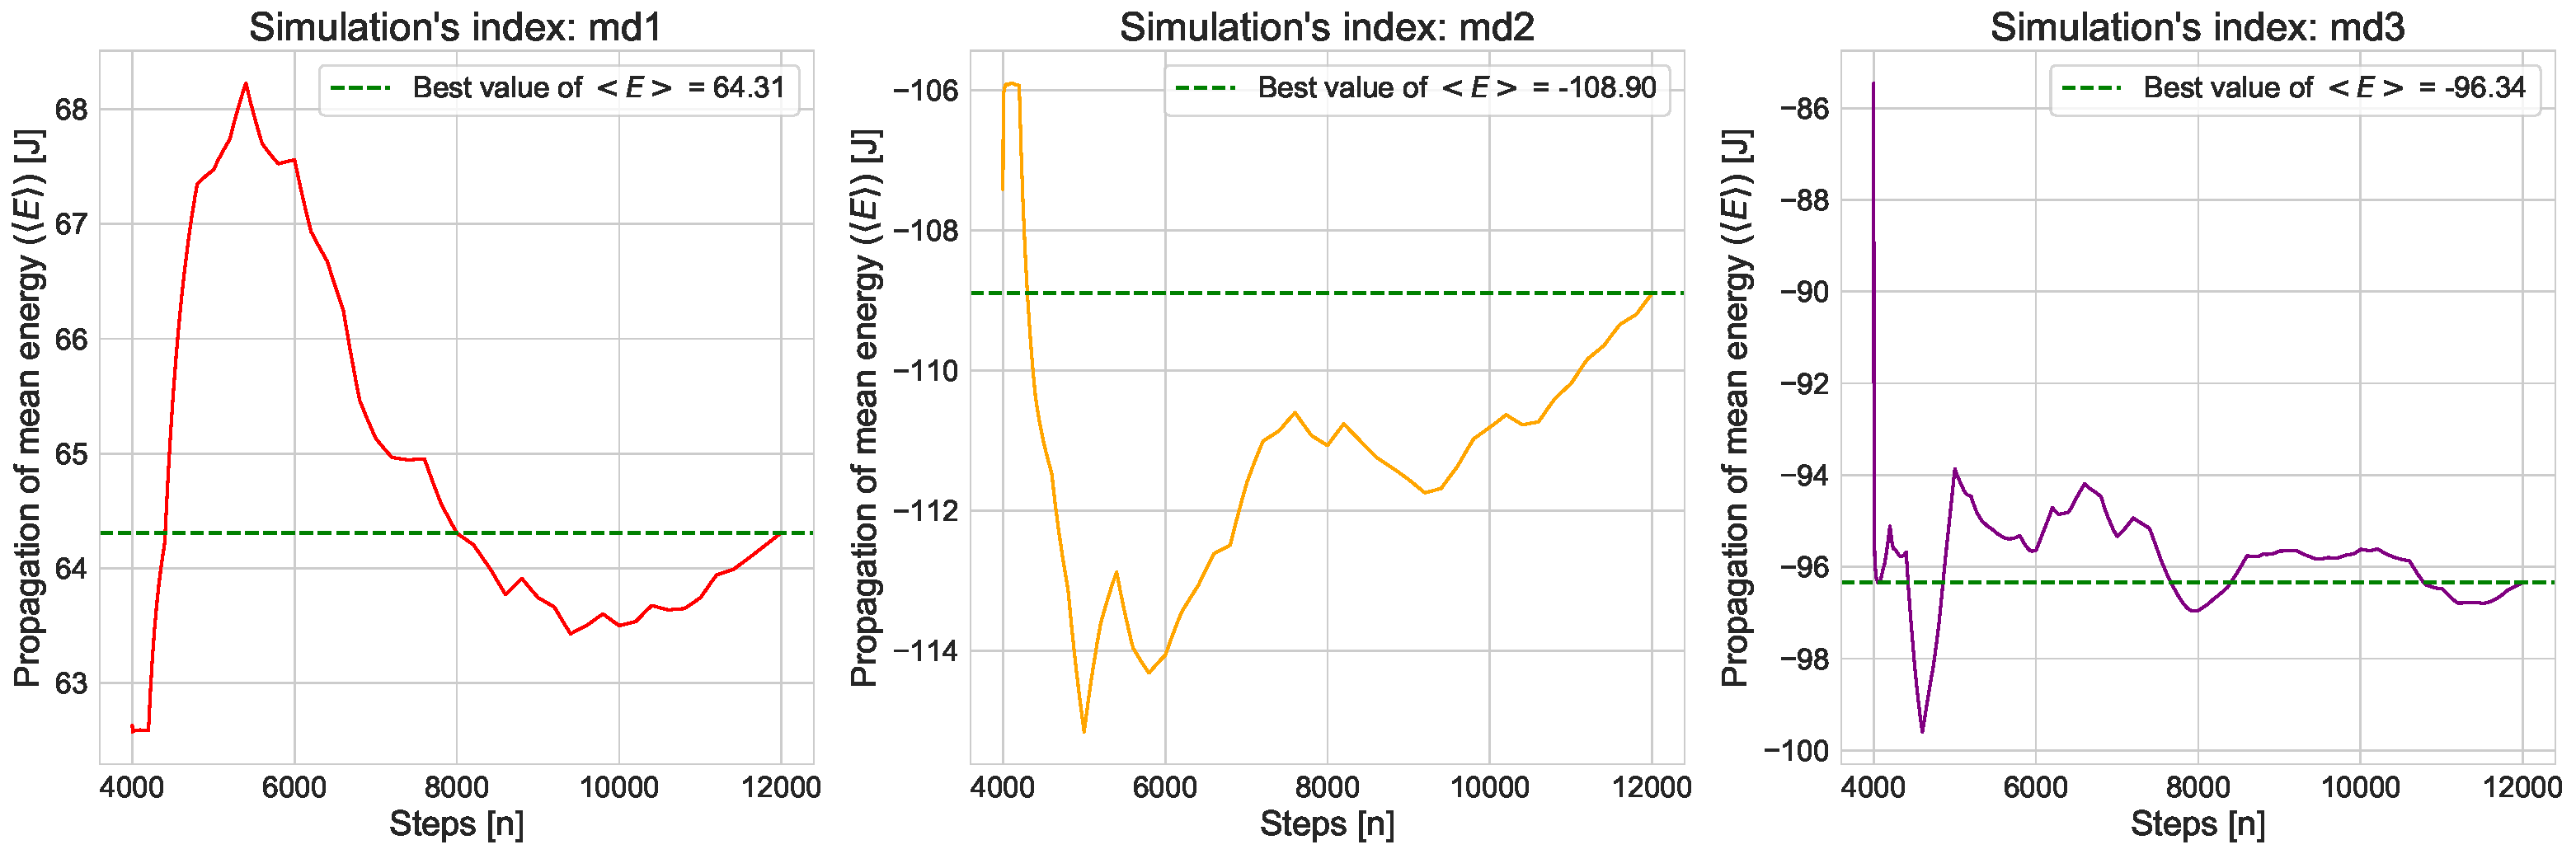
\includegraphics[width=\textwidth]{images/energy_propag_12.pdf}}
\captionof{figure}{A mérthető energia időátlaga az egyensúlyi állapotban ($\left< E \right>$) $N = 64$ részecske esetén} \label{fig:7}
\hfill \break \break
{\centering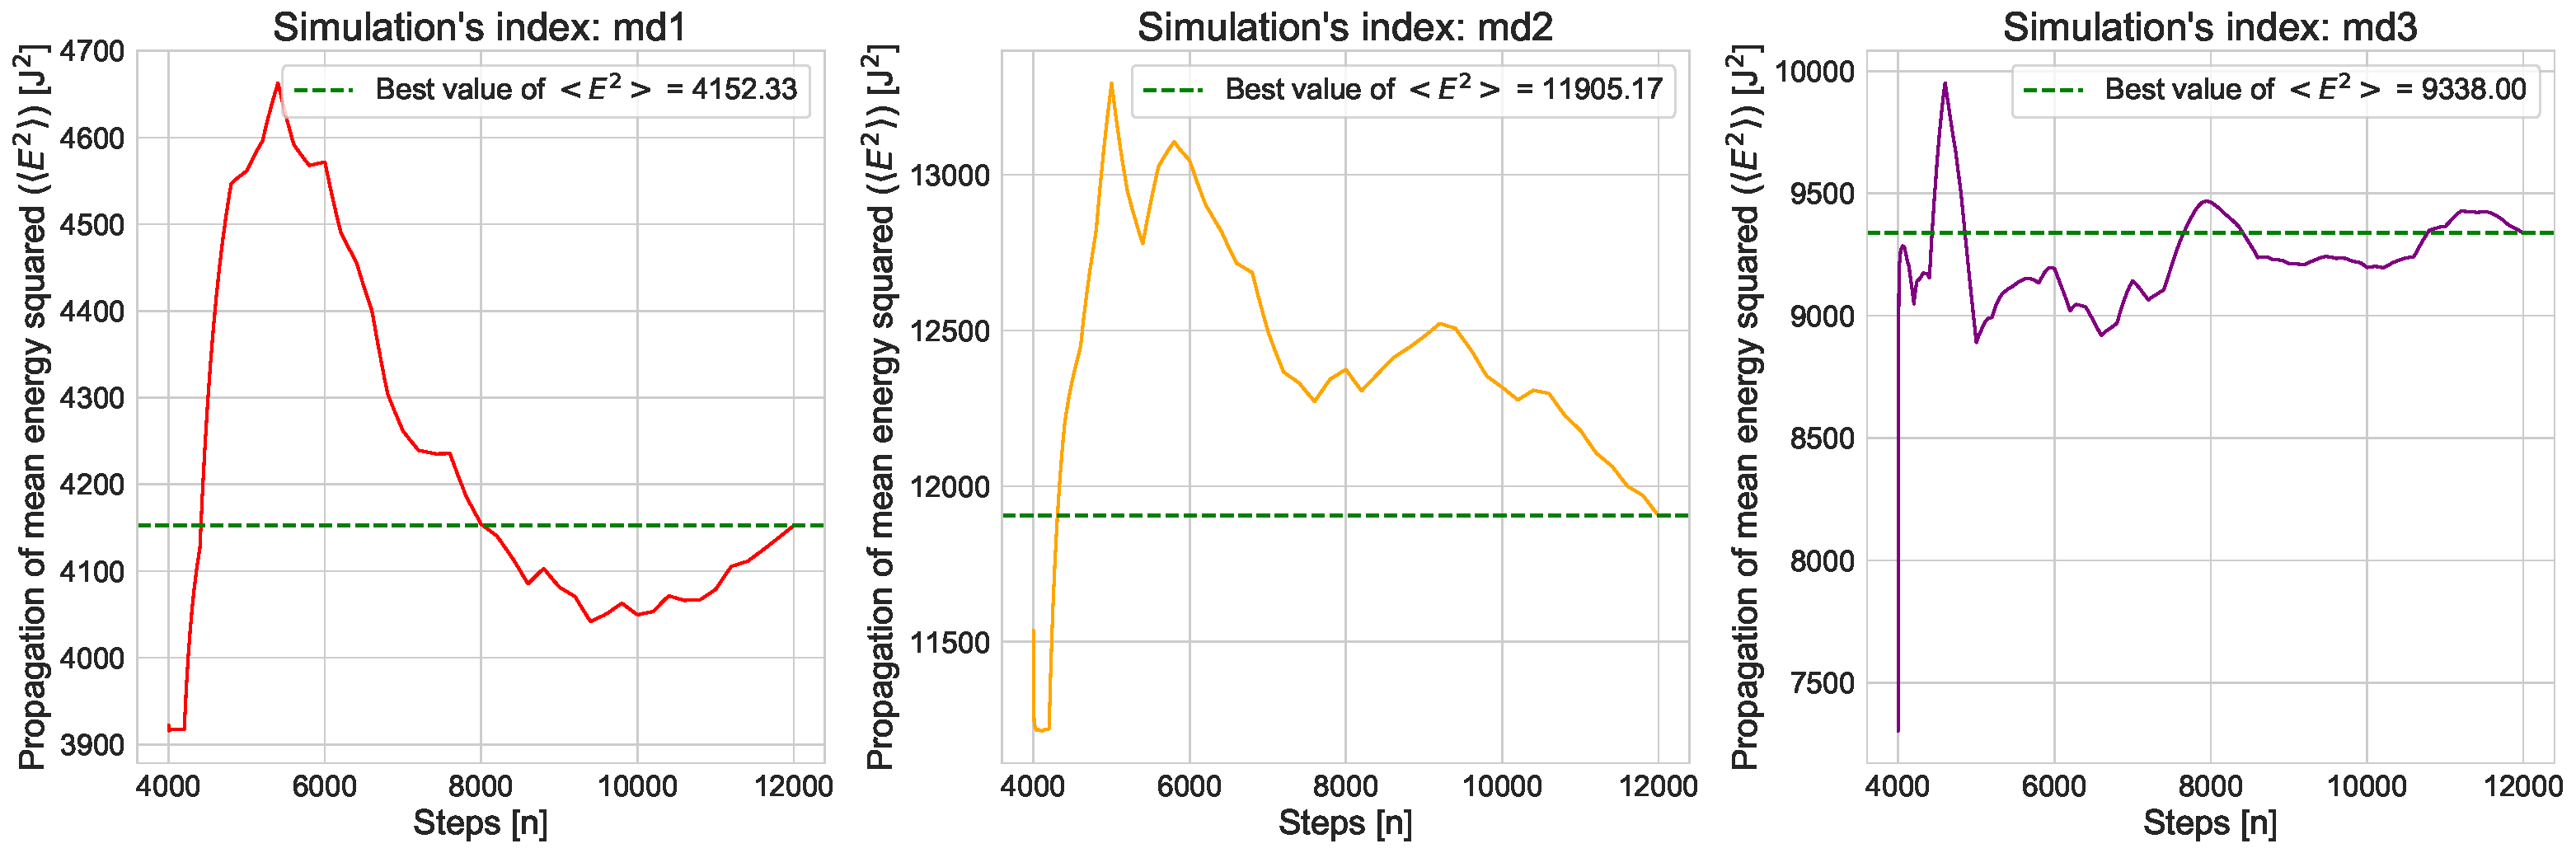
\includegraphics[width=\textwidth]{images/energy2_propag_12.pdf}}
\captionof{figure}{A mérthető energia négyzetének időátlaga az egyensúlyi állapotban ($\left< E^{2} \right>$) $N = 64$ részecske esetén} \label{fig:8}

\newpage

{\centering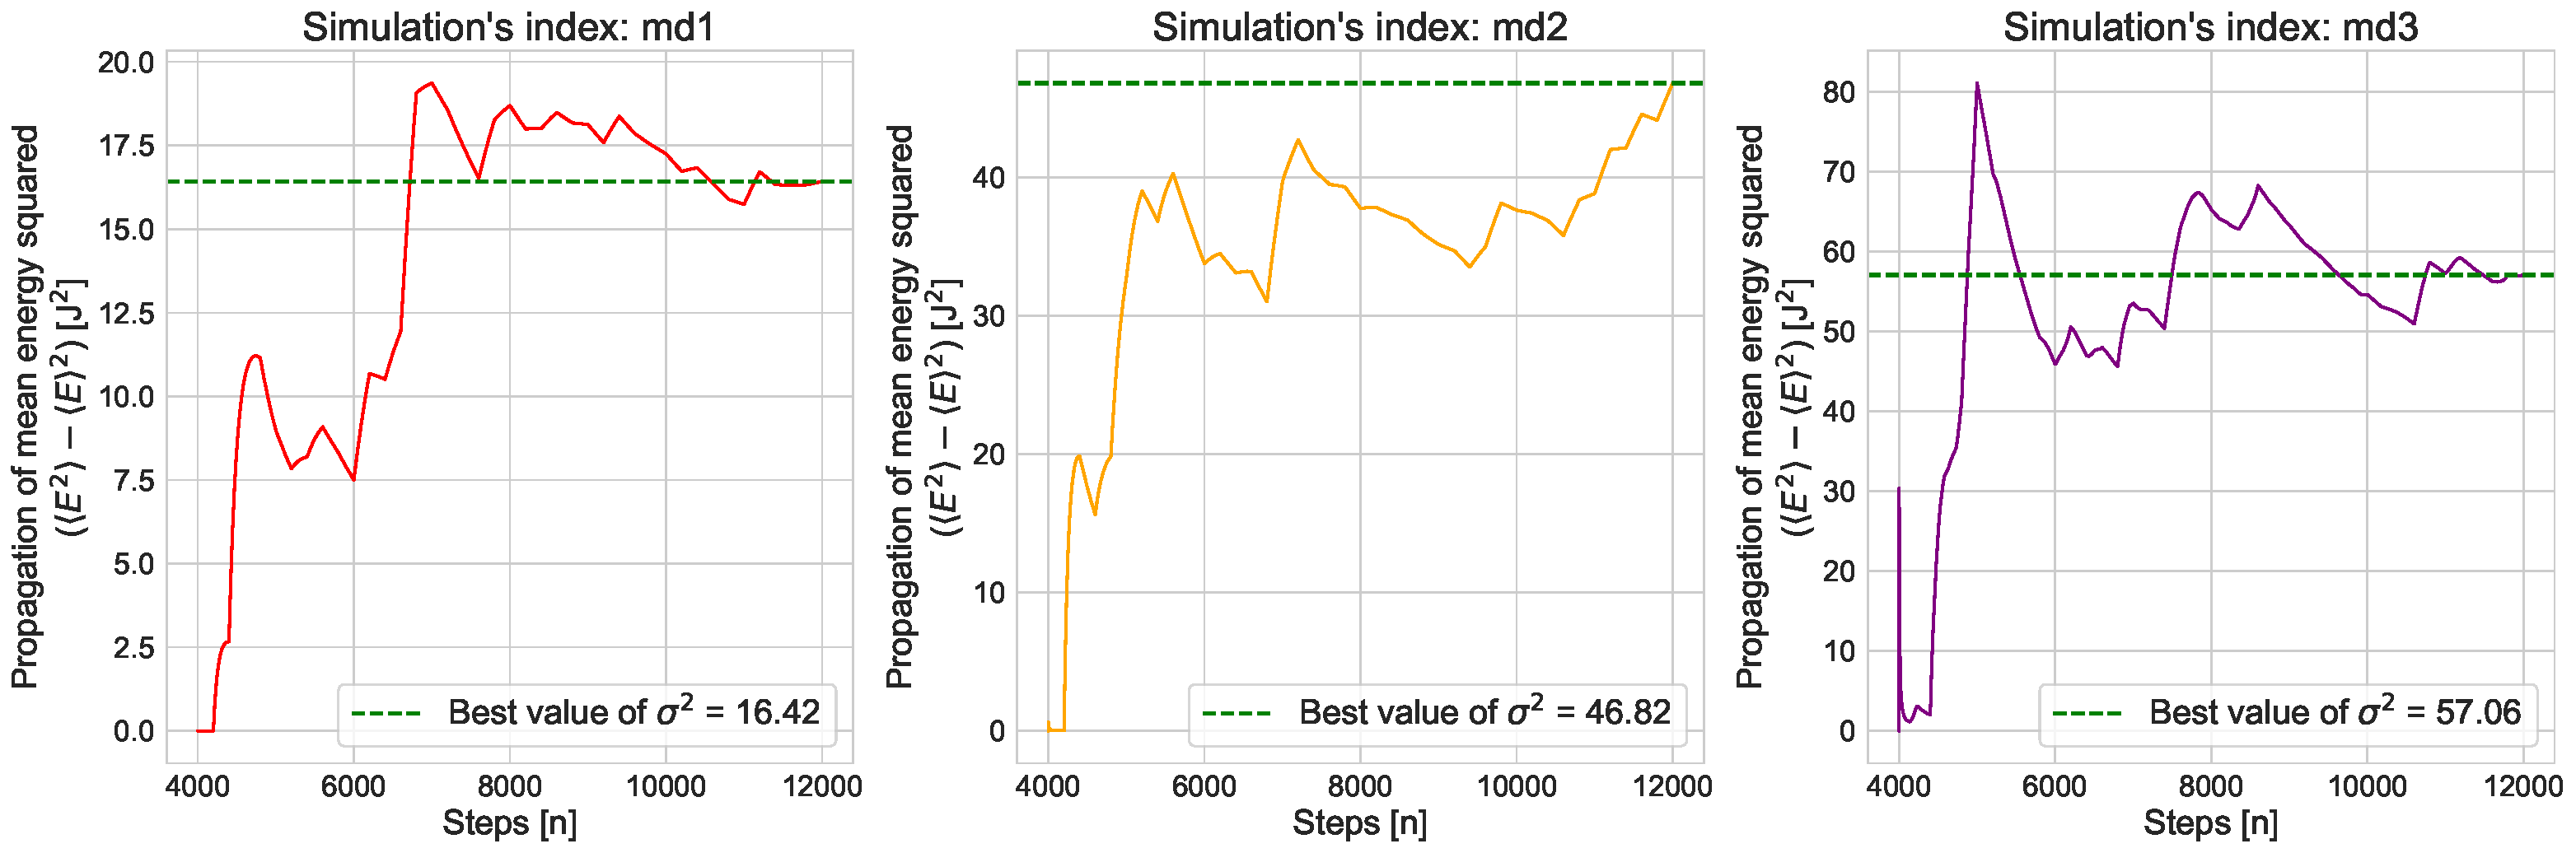
\includegraphics[width=\textwidth]{images/energy_oscill_12.pdf}}
\captionof{figure}{Az energia fluktuációja egyensúlyi állapotban ($\left< E^{2} \right> - \left< E \right>^{2}$) $N = 64$ részecske esetén} \label{fig:9}
\hfill \break \break
{\centering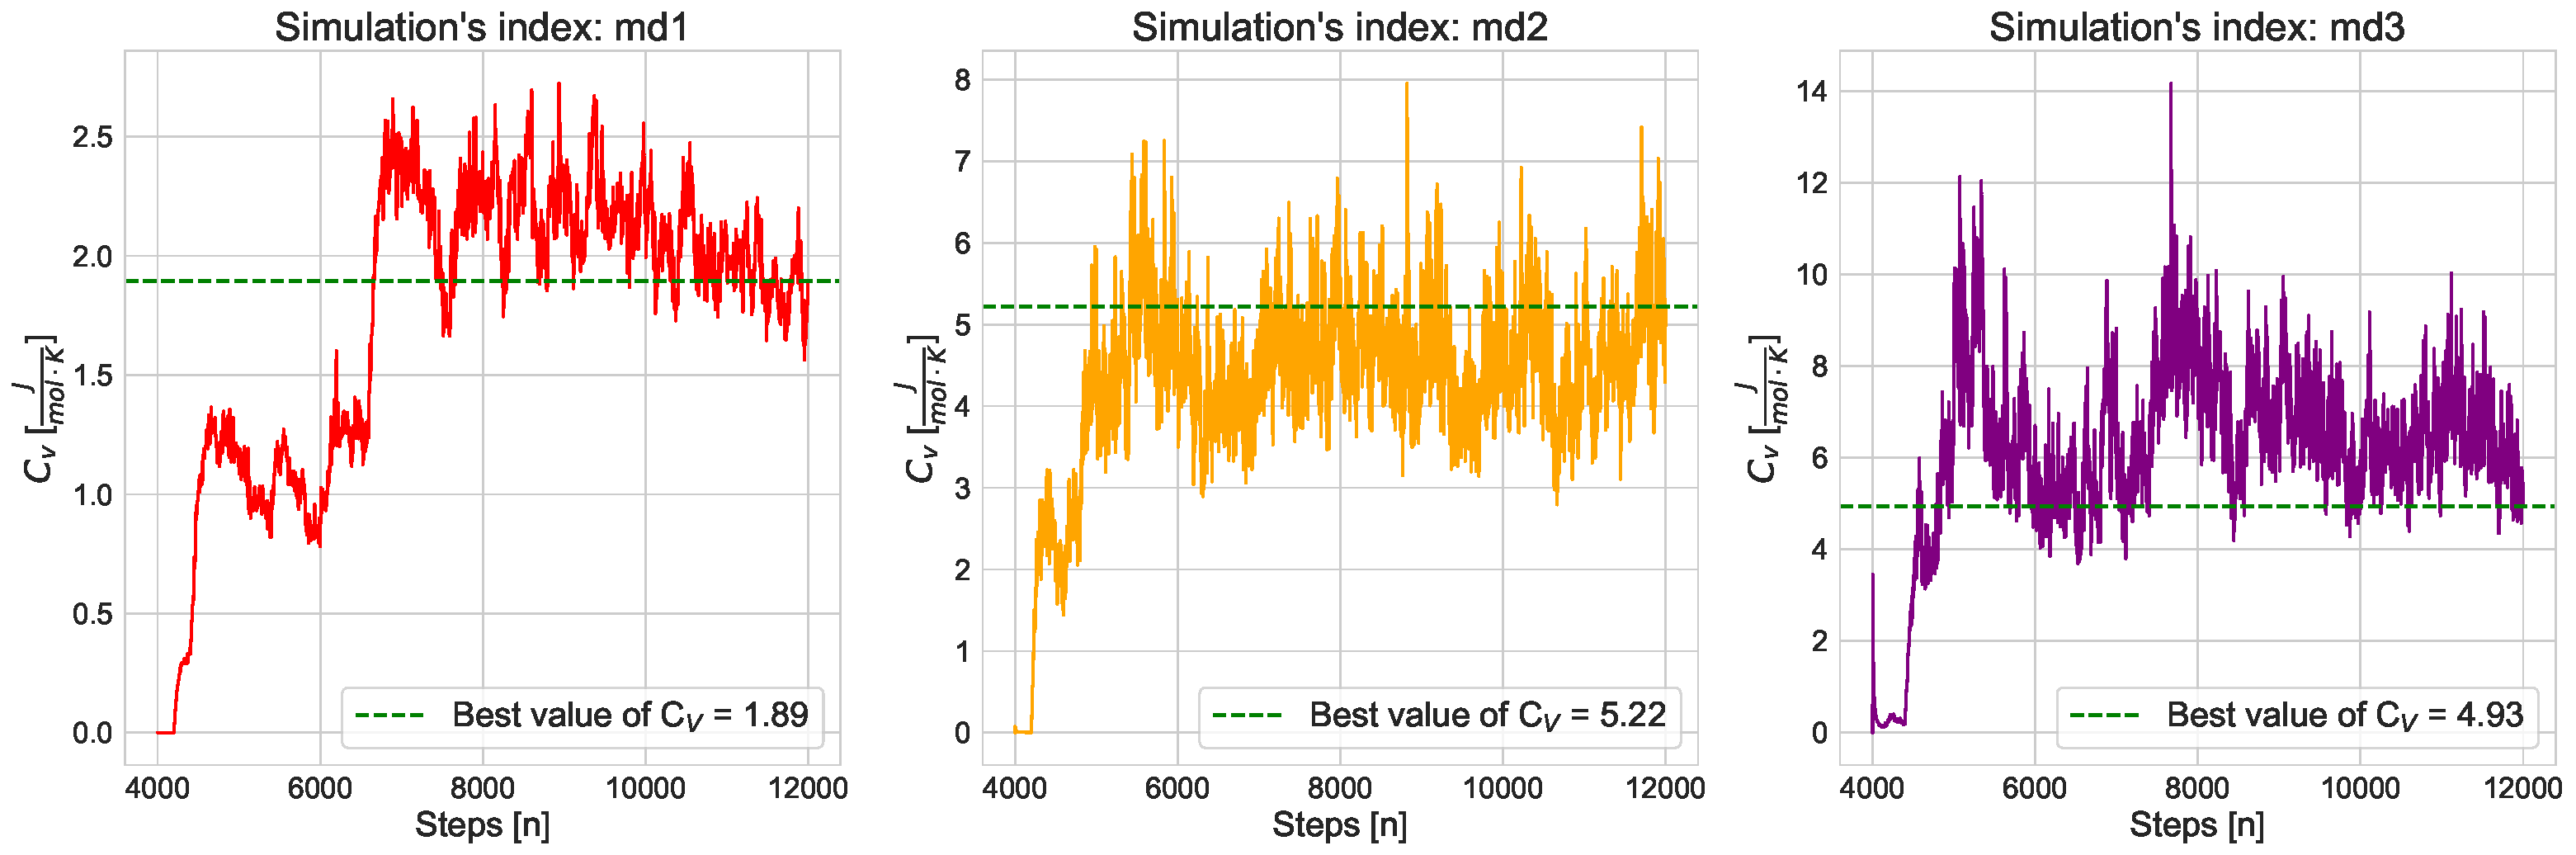
\includegraphics[width=\textwidth]{images/heat_capacity_propag_12.pdf}}
\captionof{figure}{A hőkapacitás közelítése egyensúlyi helyzetben $N = 64$ részecske esetén} \label{fig:10}
\hfill \break \break
{\centering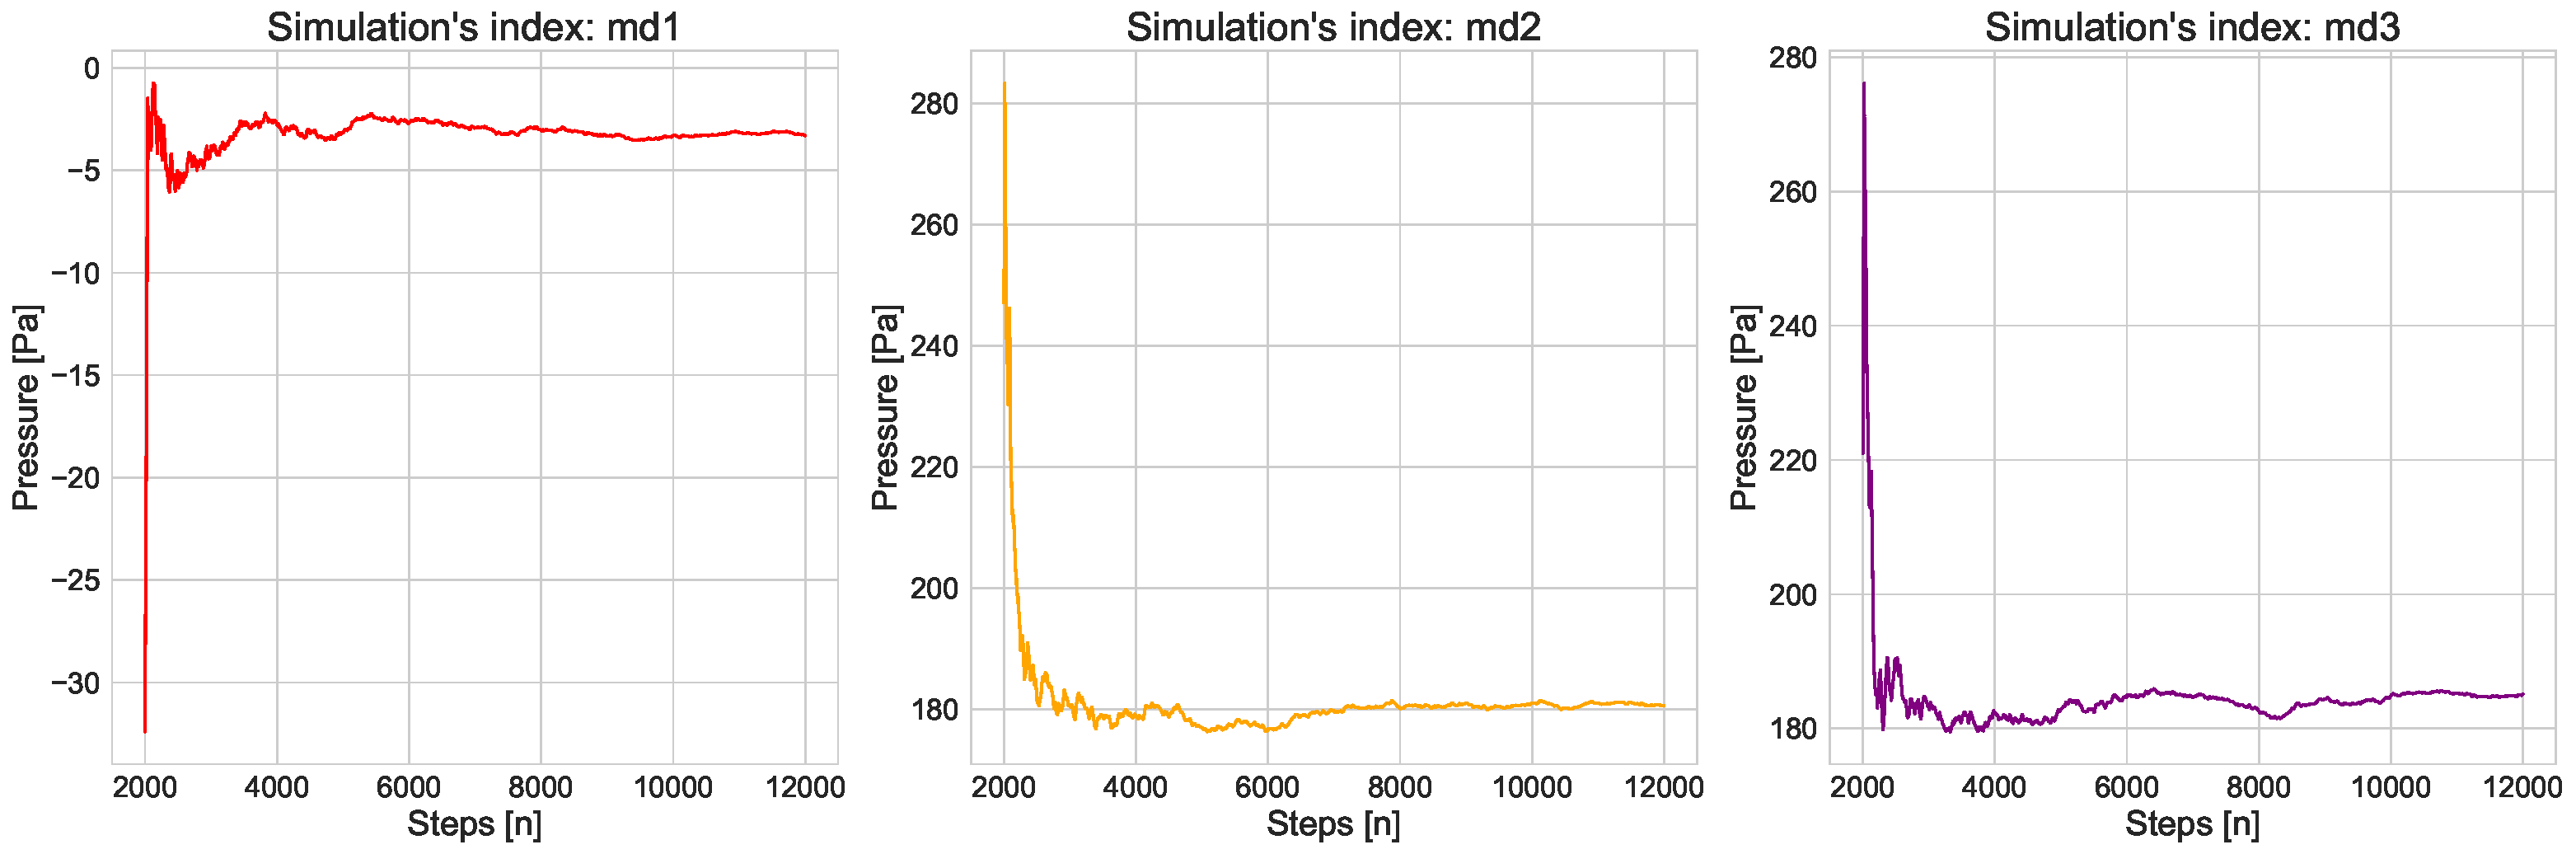
\includegraphics[width=\textwidth]{images/PV_12.pdf}}
\captionof{figure}{A $PV$ nyomás $\times$ térfogat érték ábrázolása, $N = 64$ részecske esetén} \label{fig:11}
\hfill \break \break
{\centering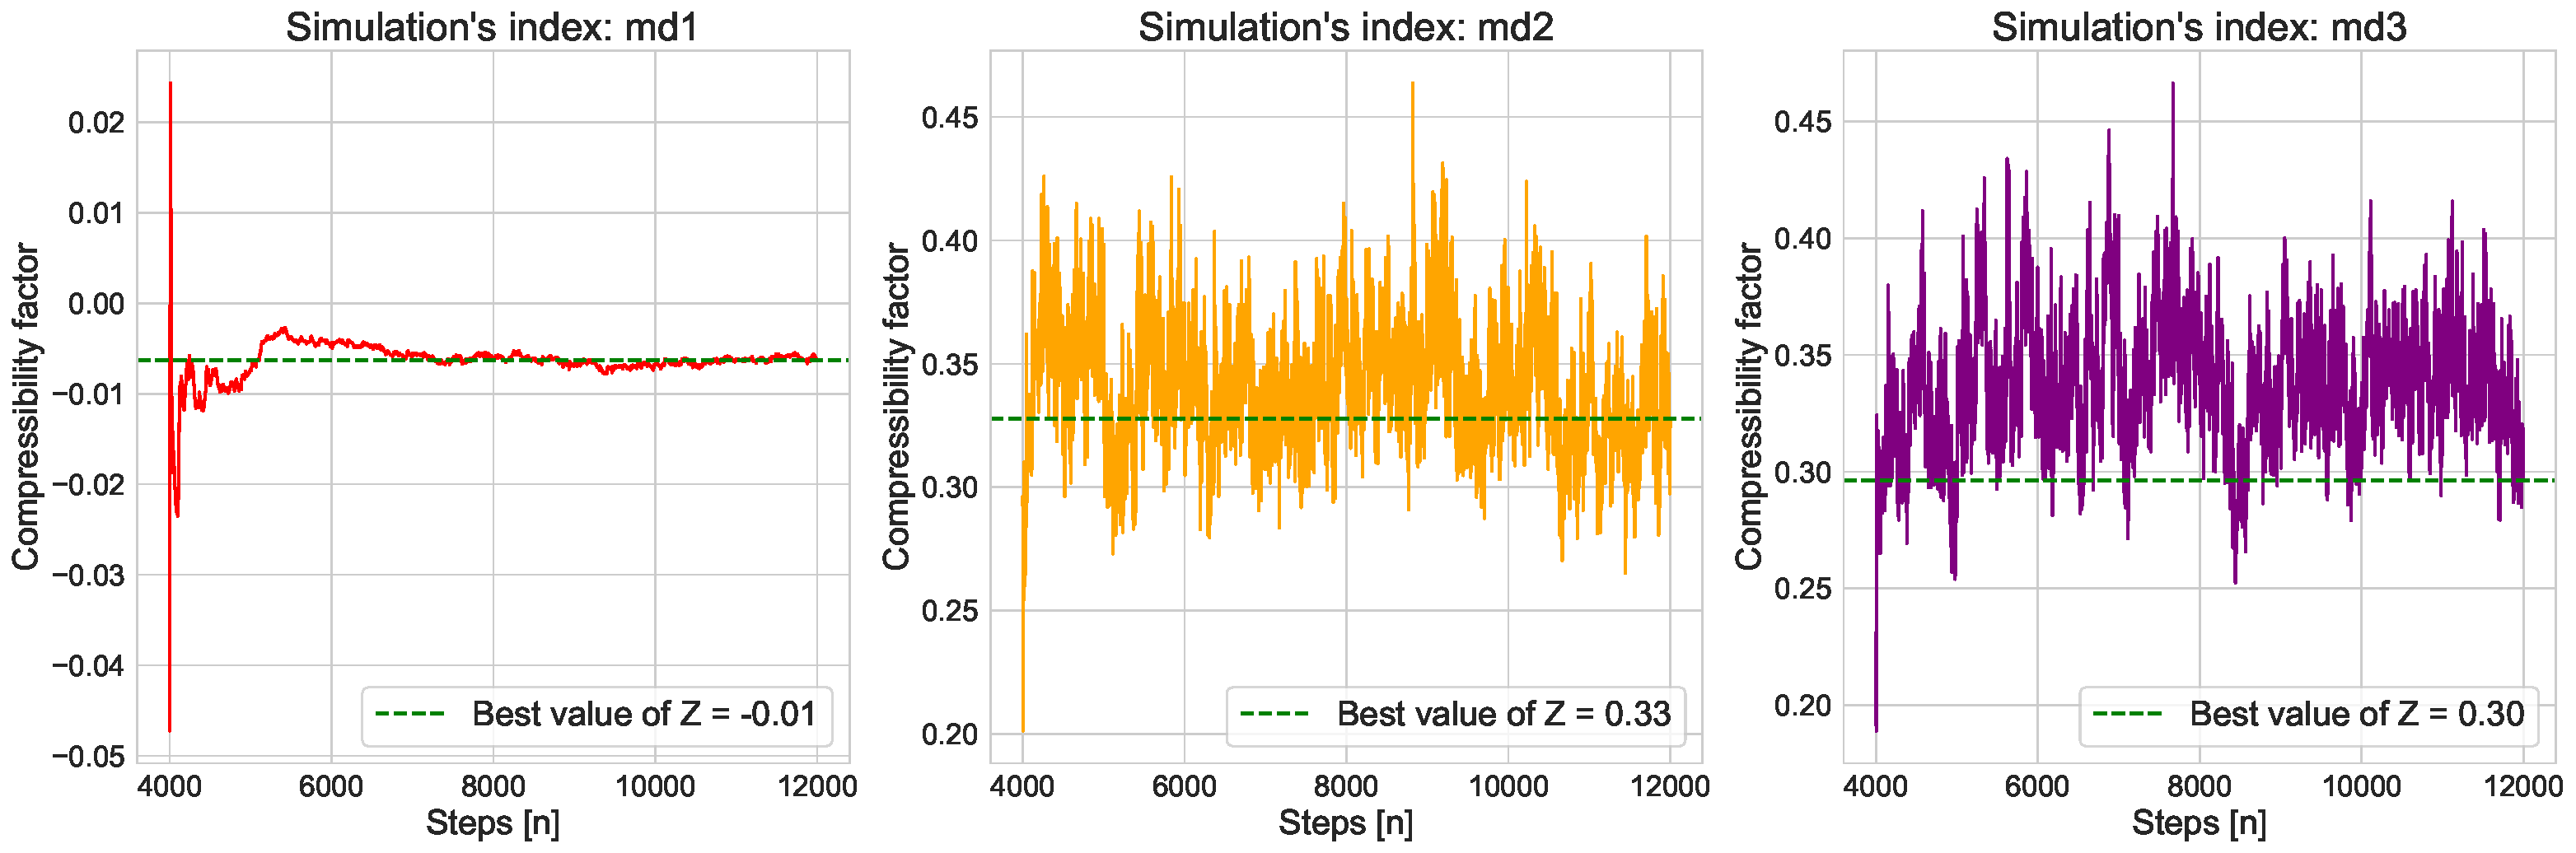
\includegraphics[width=\textwidth]{images/Z_12.pdf}}
\captionof{figure}{A kompresszibilitási faktor közelítése $N = 64$ részecske esetén} \label{fig:12}

\newpage

\subsection*{A.1.2\ \ Mérendő mennyiségek adatai $n=24000$ lépés esetén}

{\centering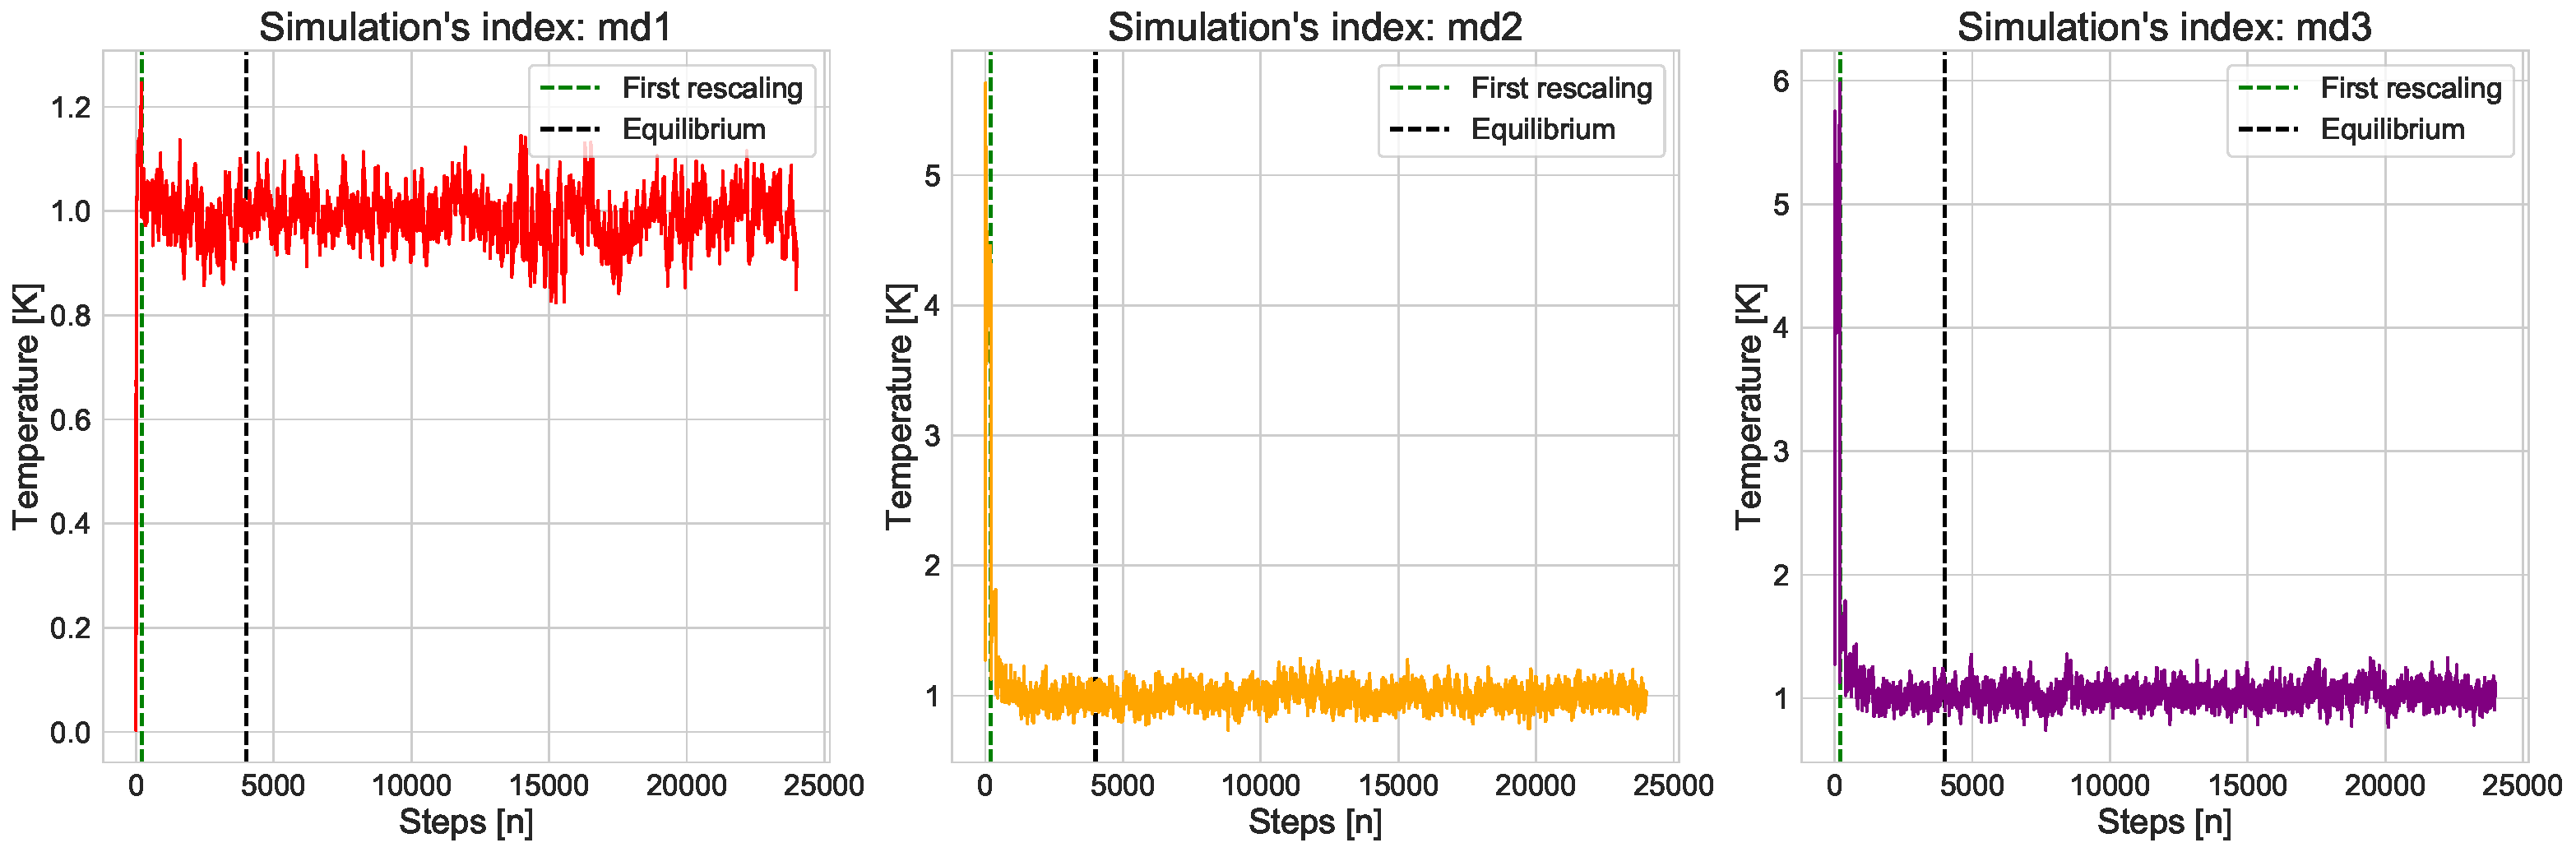
\includegraphics[width=\textwidth]{images/instantaneous_temperatures_24.pdf}}
\captionof{figure}{Pillanatnyi hőmérsékletek zárt rendszerben, $N = 64$ részecske esetén} \label{fig:13}
\hfill \break \break
{\centering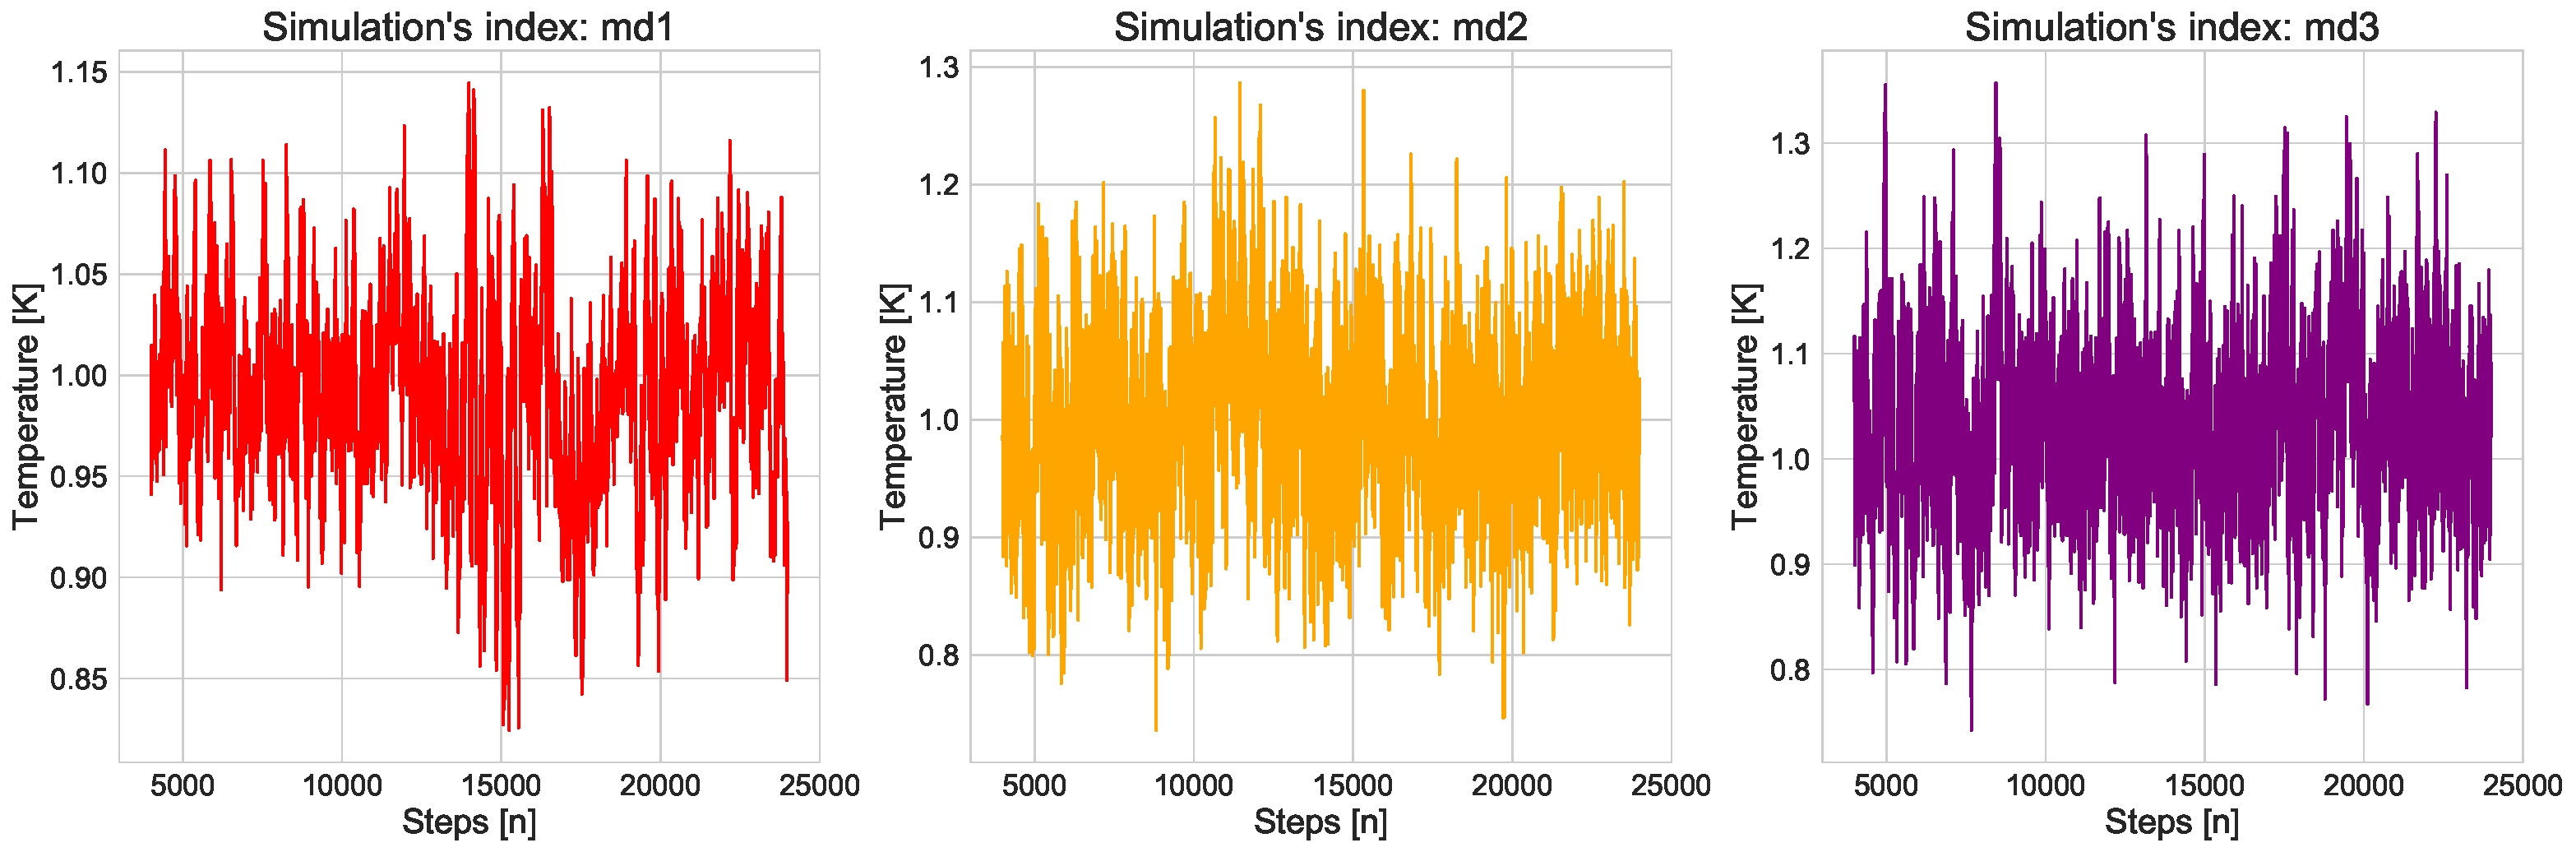
\includegraphics[width=\textwidth]{images/instantaneous_temperatures_equi_24.pdf}}
\captionof{figure}{Pillanatnyi hőmérsékletek zárt rendszerben, az egyensúlyi állapotban, $N = 64$ részecske esetén} \label{fig:14}
\hfill \break \break
{\centering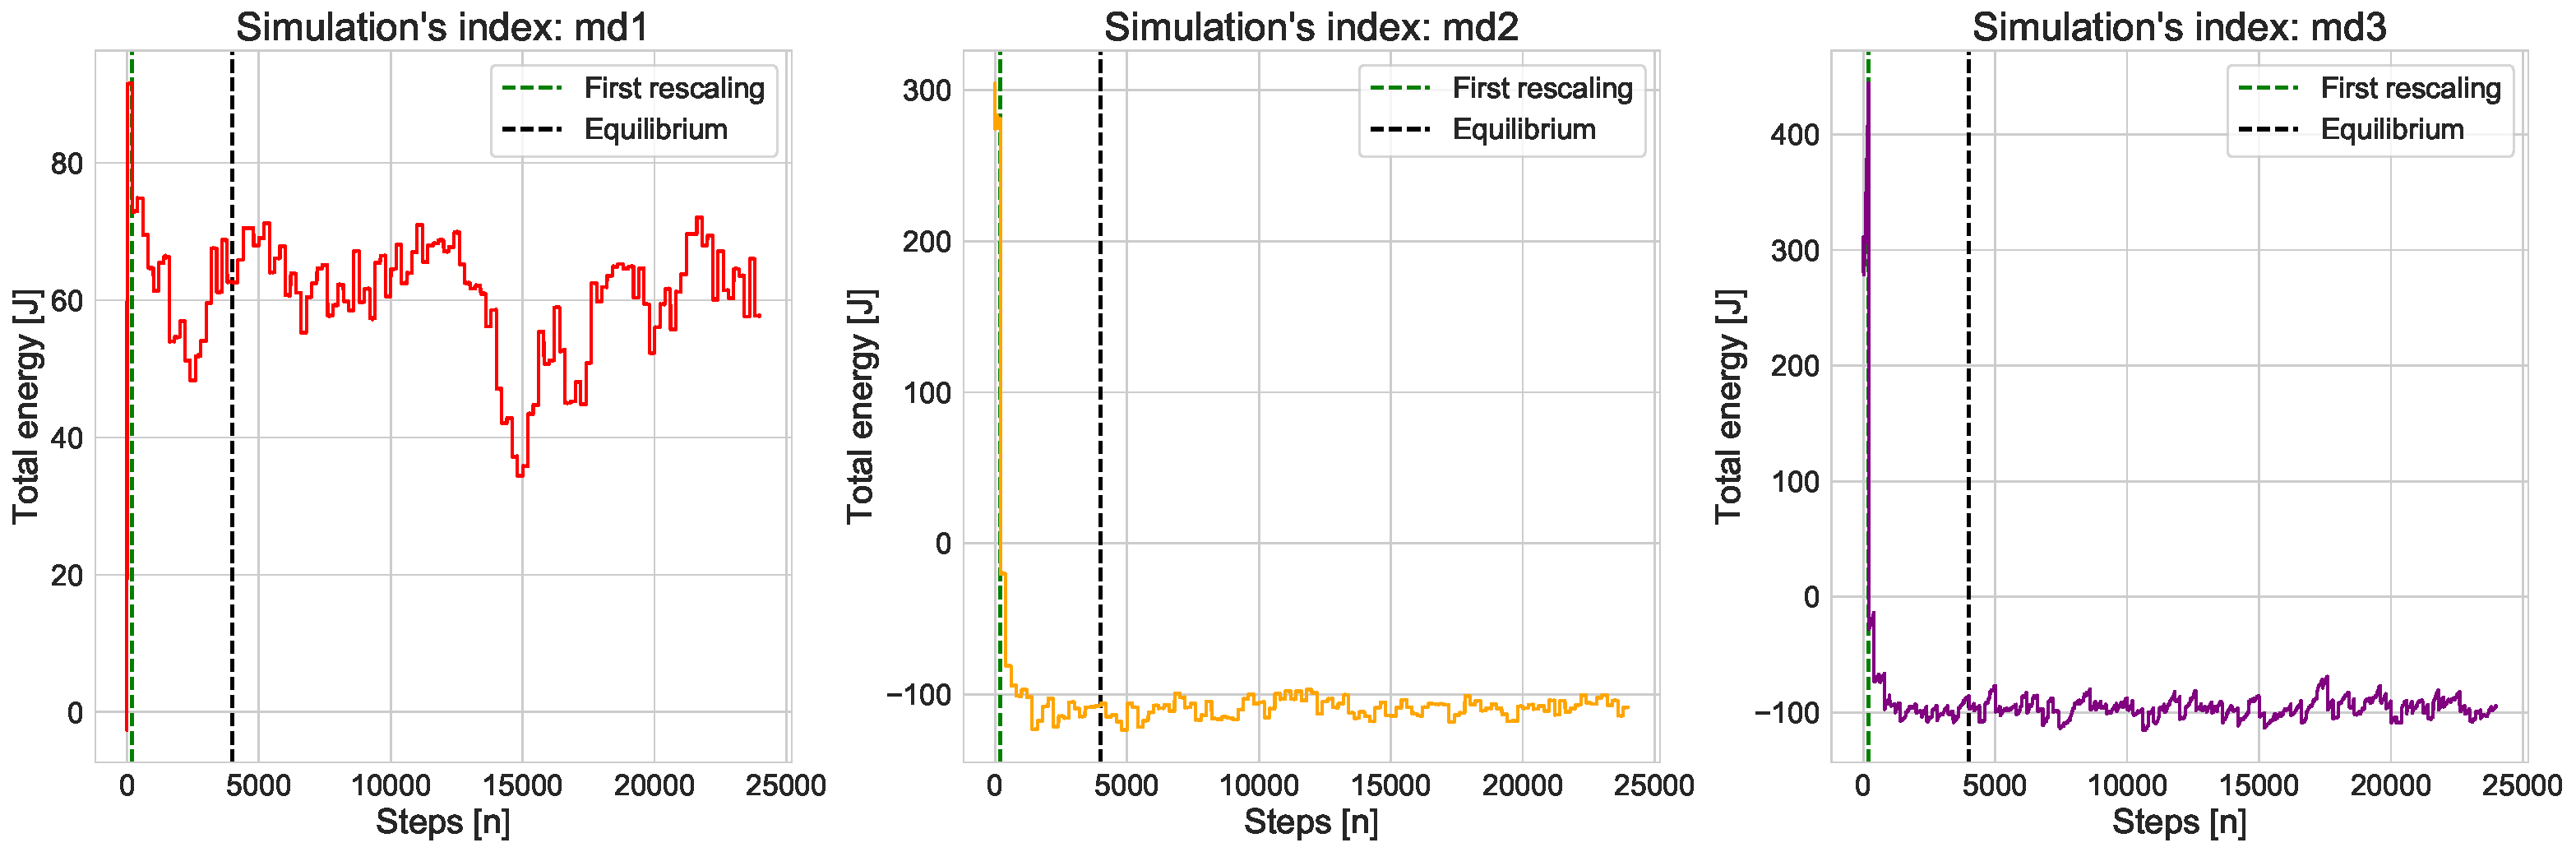
\includegraphics[width=\textwidth]{images/total_energy_24.pdf}}
\captionof{figure}{A zárt rendszer teljes energiája $N = 64$ részecske esetén} \label{fig:15}
\hfill \break \break
{\centering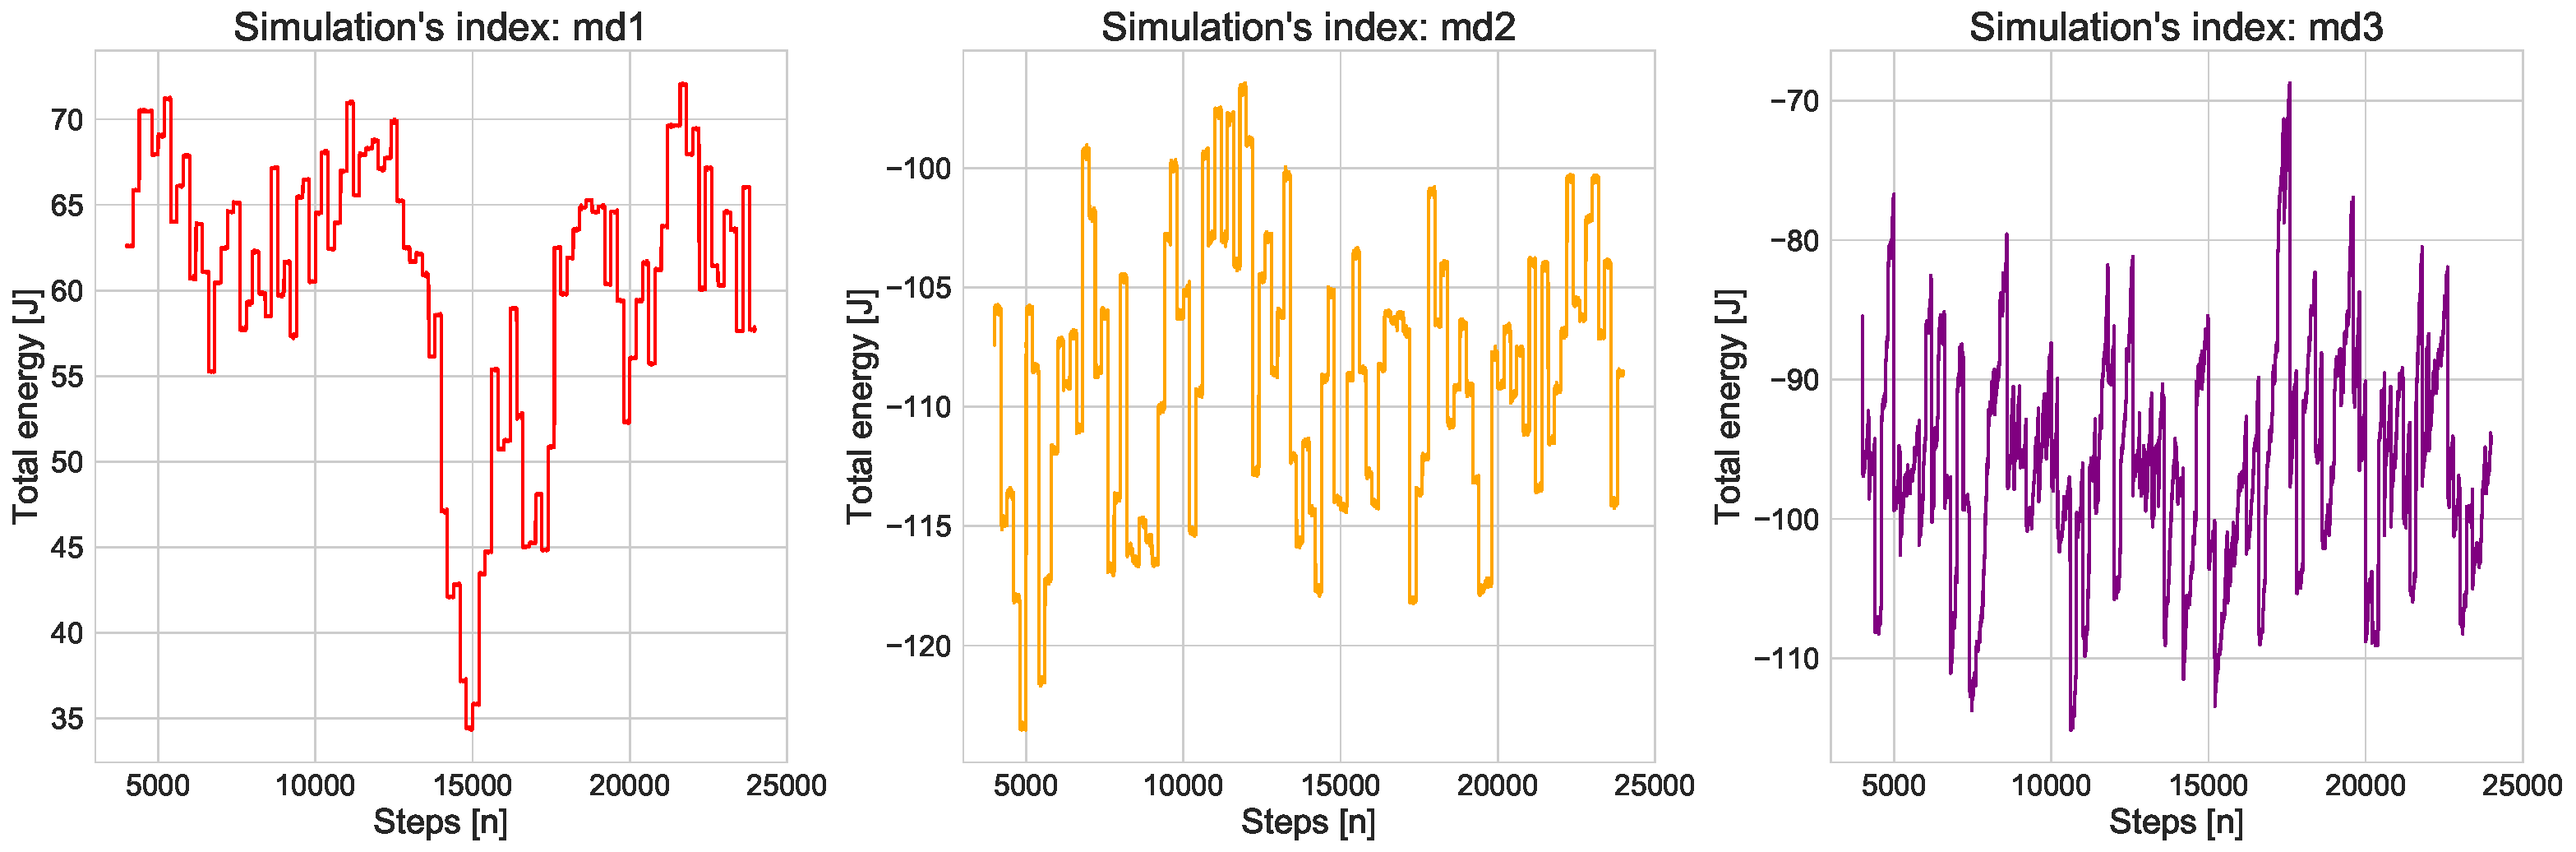
\includegraphics[width=\textwidth]{images/total_energy_equi_24.pdf}}
\captionof{figure}{A zárt rendszer teljes energiája az egyensúlyi állapotban $N = 64$ részecske esetén} \label{fig:16}

\newpage

{\centering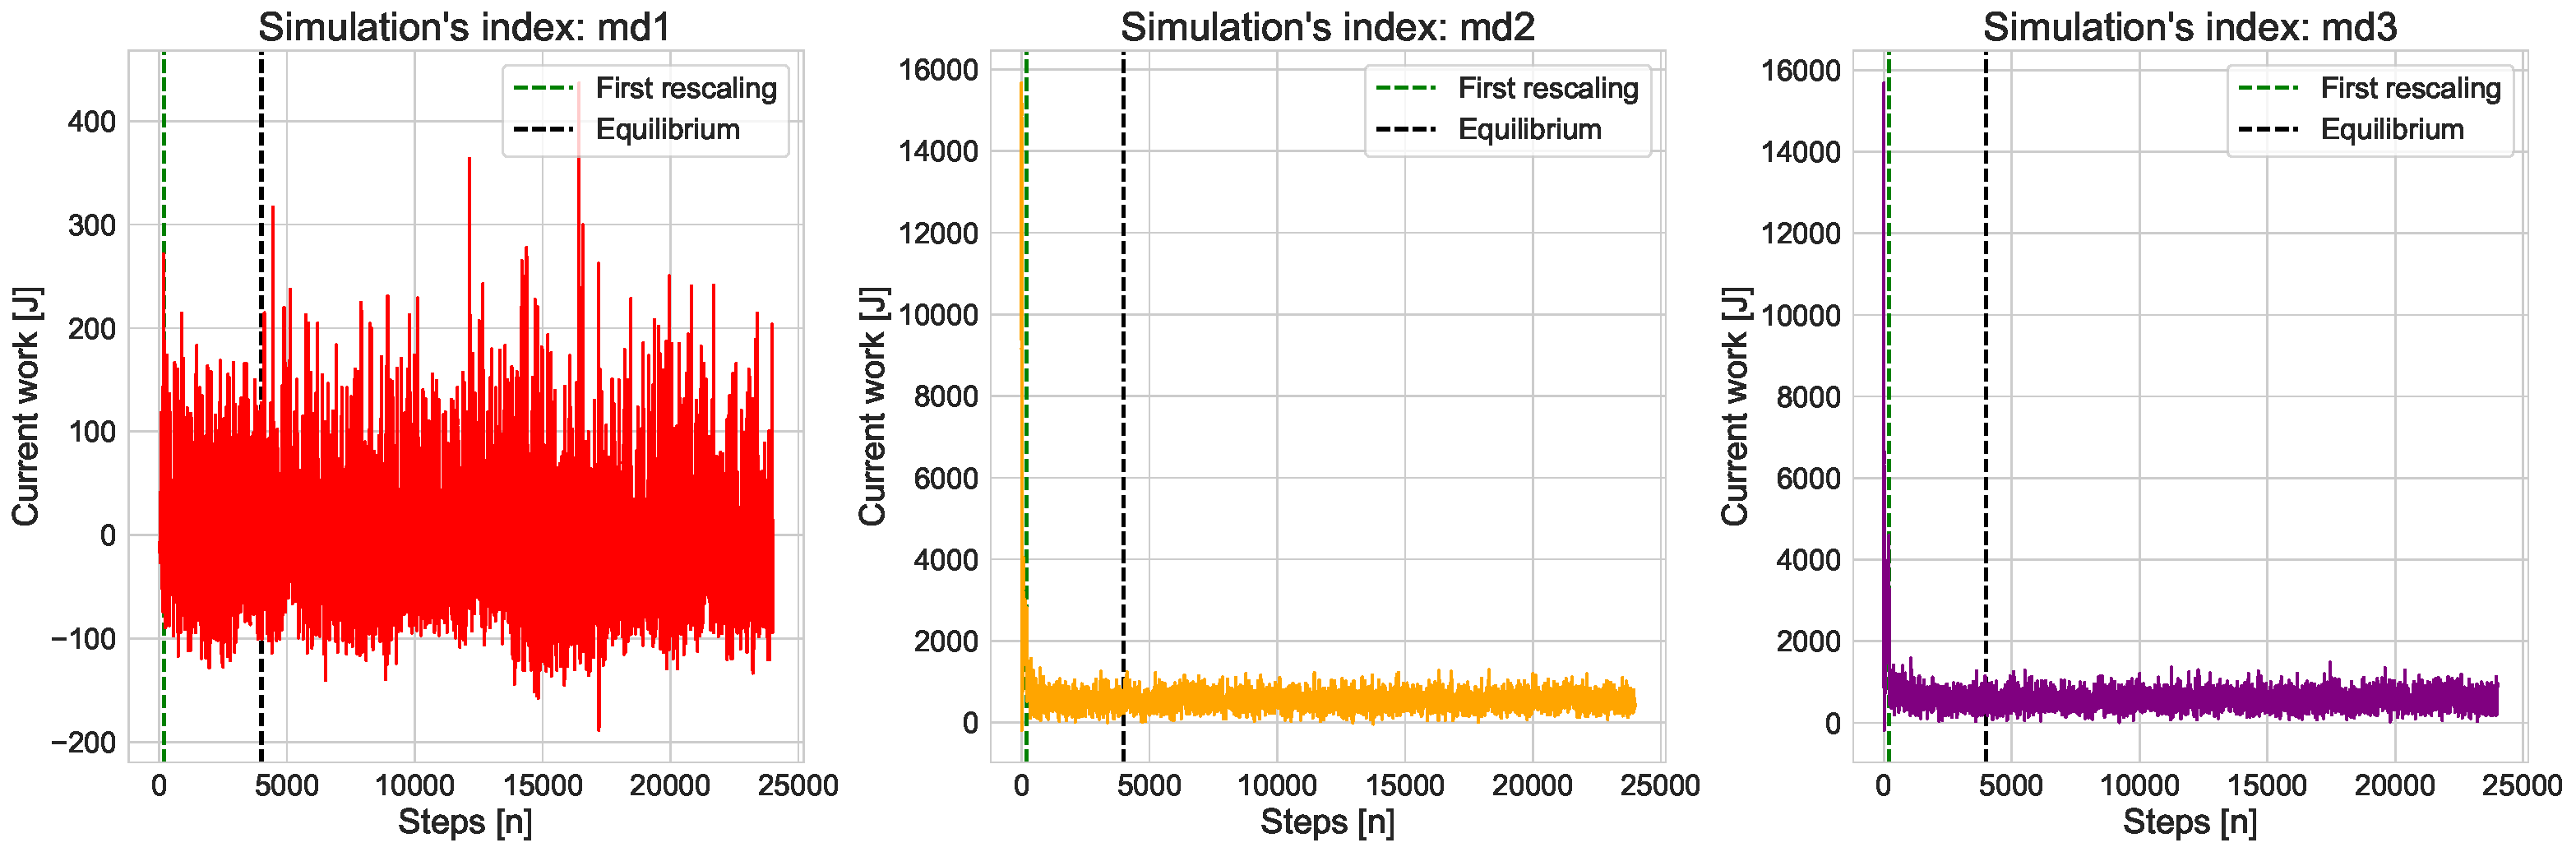
\includegraphics[width=\textwidth]{images/virial_24.pdf}}
\captionof{figure}{A mérhető munka időátlaga ($\left< \sum_{i < j} \boldsymbol{r}_{ij} \cdot \boldsymbol{F}_{ij} \right>$) $N = 64$ részecske esetén} \label{fig:17}
\hfill \break \break
{\centering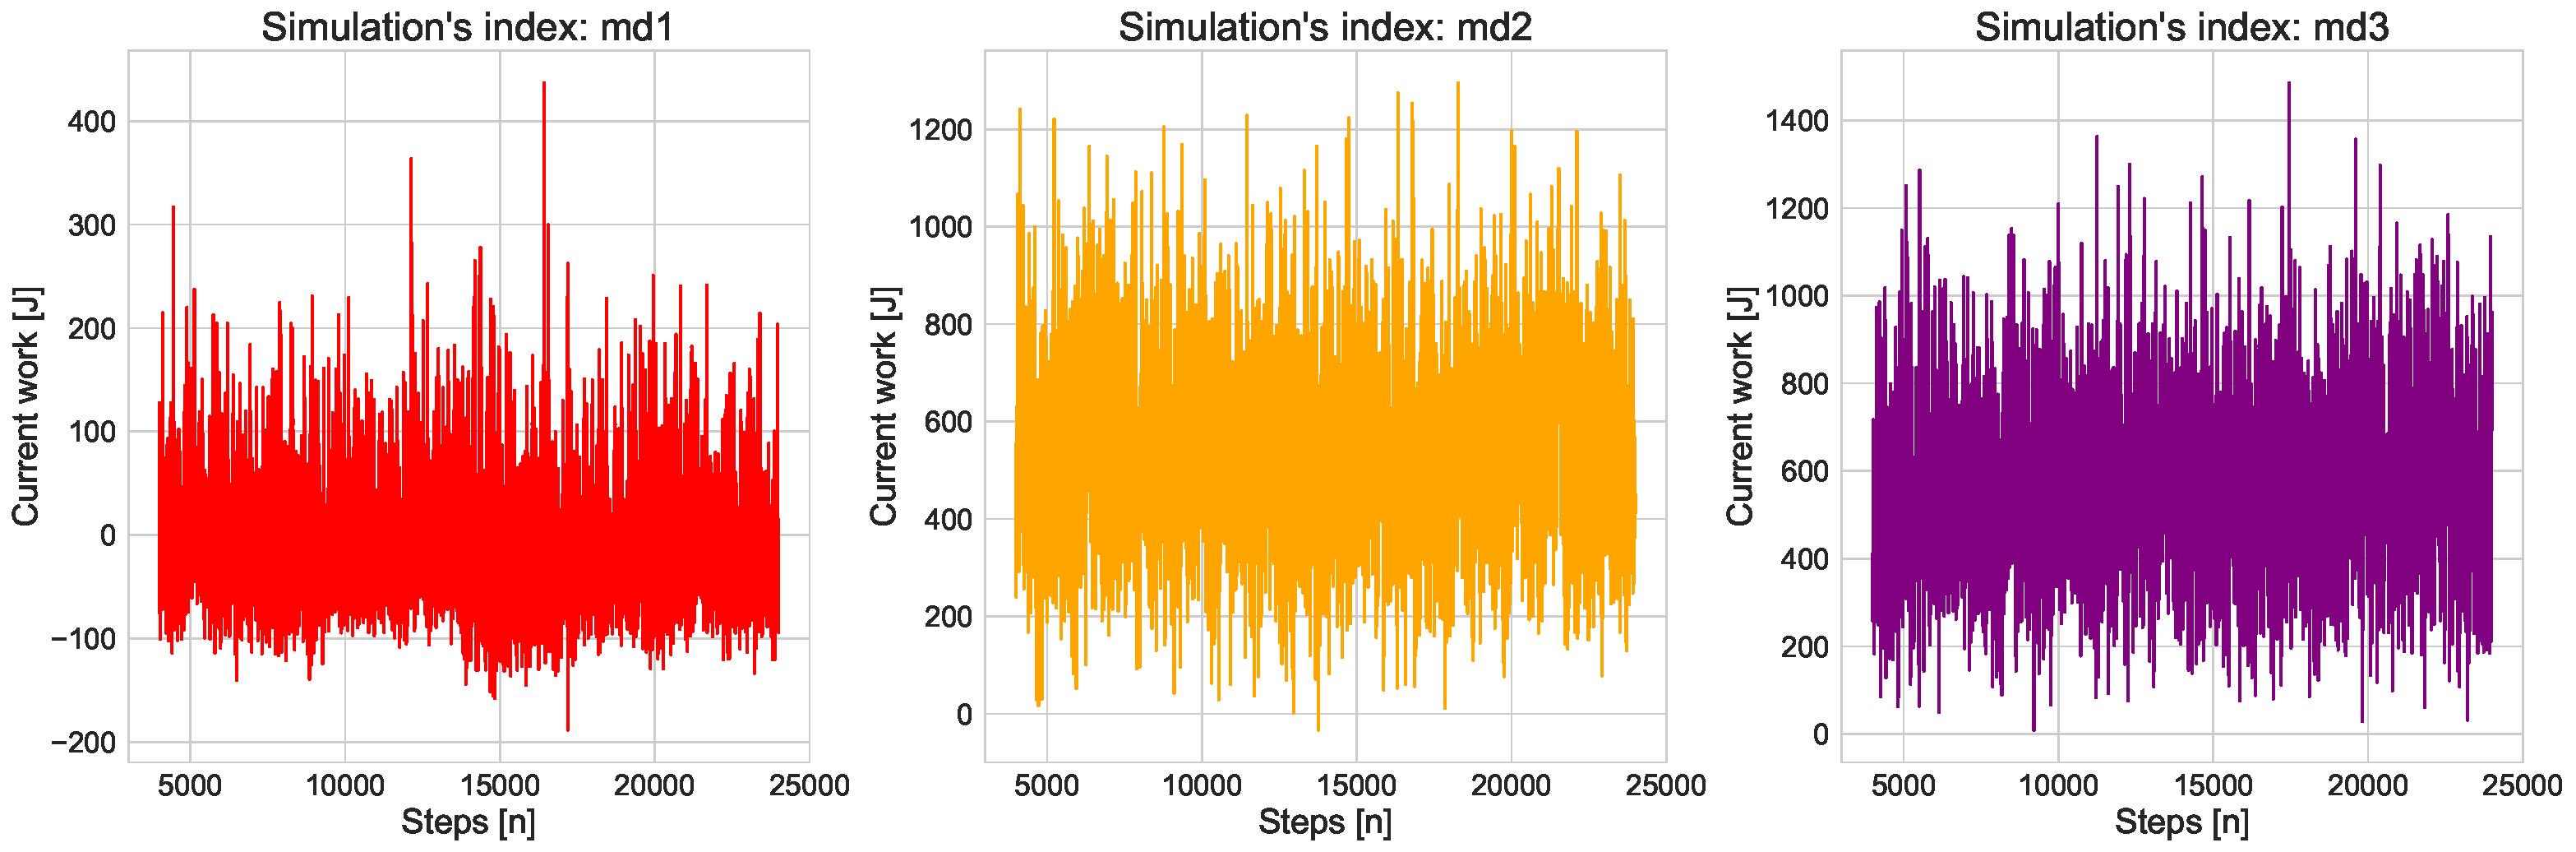
\includegraphics[width=\textwidth]{images/virial_equi_24.pdf}}
\captionof{figure}{A mérhető munka időátlaga az egyensúlyi állapotban ($\left< \sum_{i < j} \boldsymbol{r}_{ij} \cdot \boldsymbol{F}_{ij} \right>$) $N = 64$ részecske esetén} \label{fig:18}
{\centering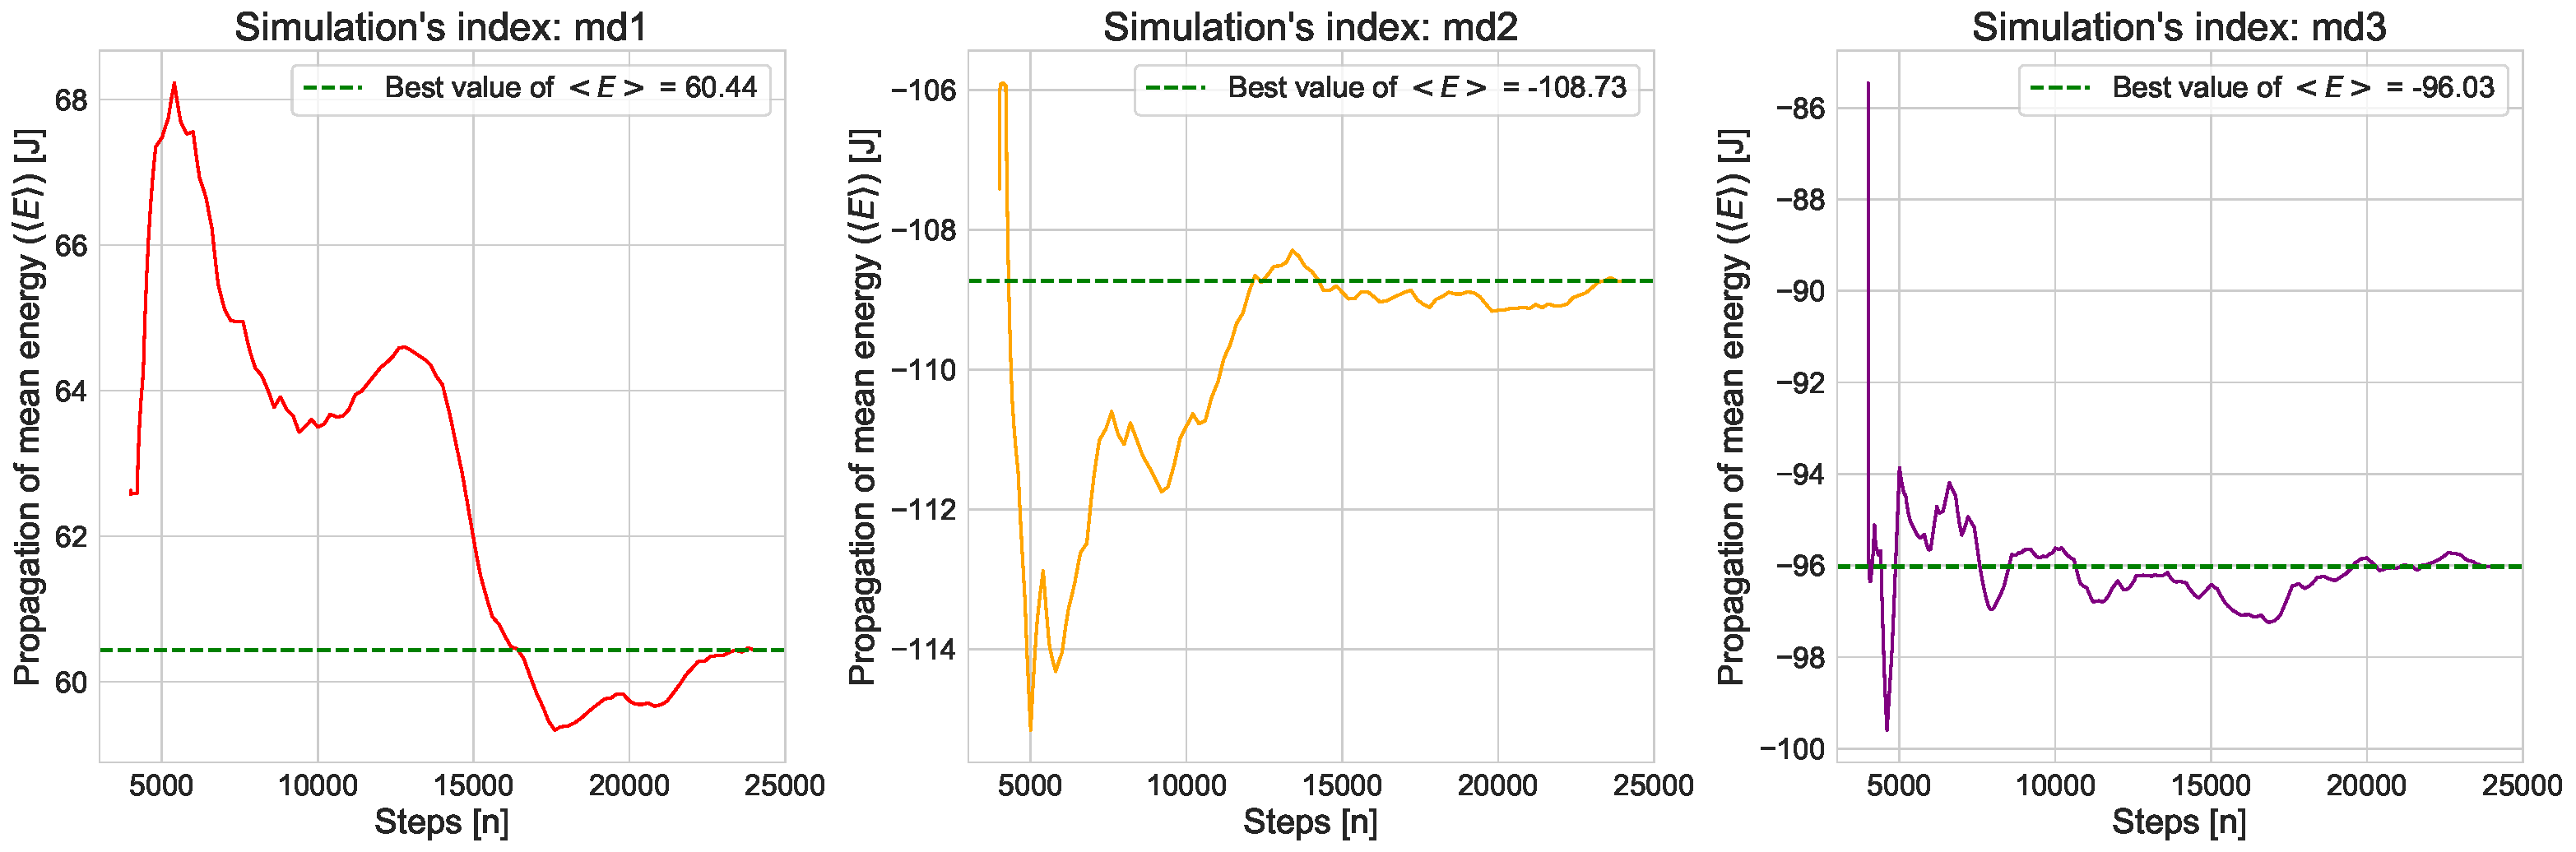
\includegraphics[width=\textwidth]{images/energy_propag_24.pdf}}
\captionof{figure}{A mérthető energia időátlaga az egyensúlyi állapotban ($\left< E \right>$) $N = 64$ részecske esetén} \label{fig:19}
\hfill \break \break
{\centering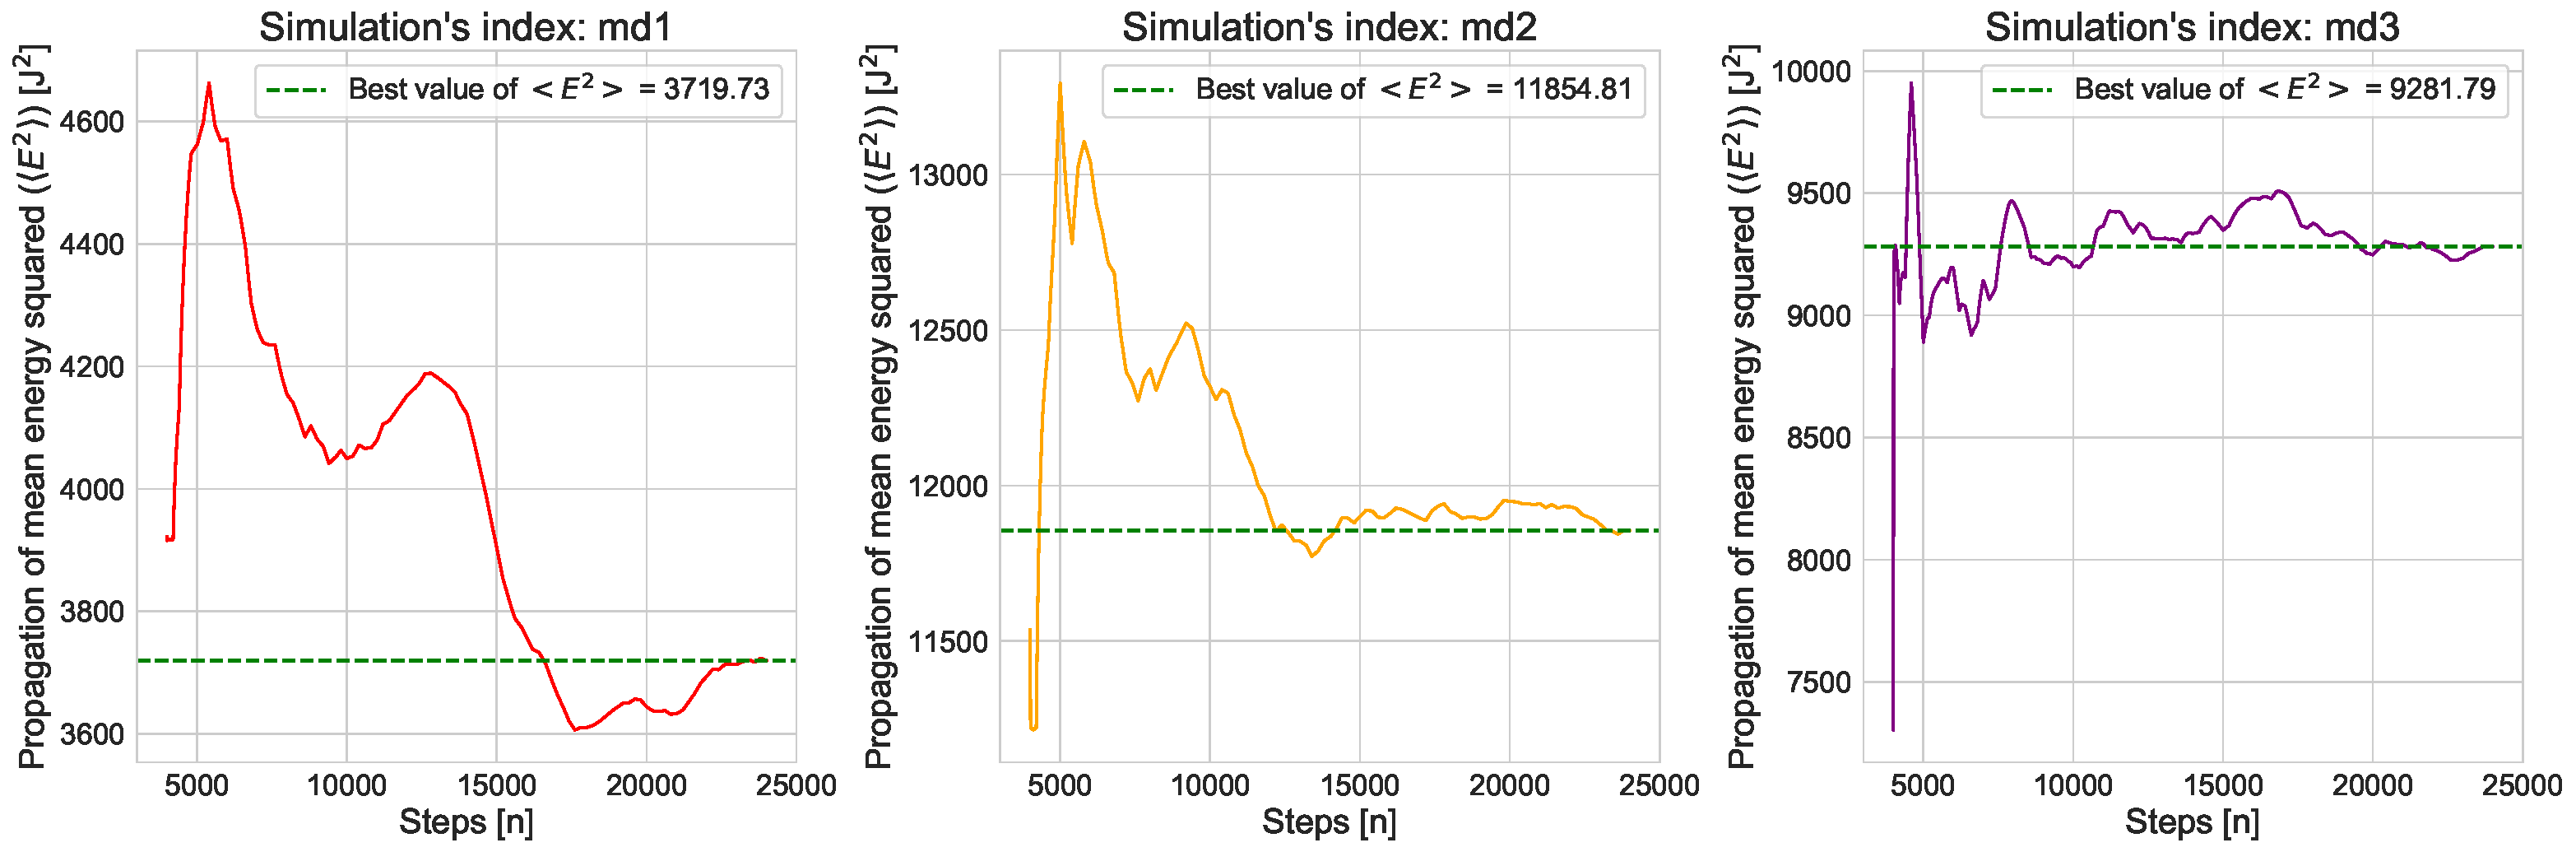
\includegraphics[width=\textwidth]{images/energy2_propag_24.pdf}}
\captionof{figure}{A mérthető energia négyzetének időátlaga az egyensúlyi állapotban ($\left< E^{2} \right>$) $N = 64$ részecske esetén} \label{fig:20}

\newpage

{\centering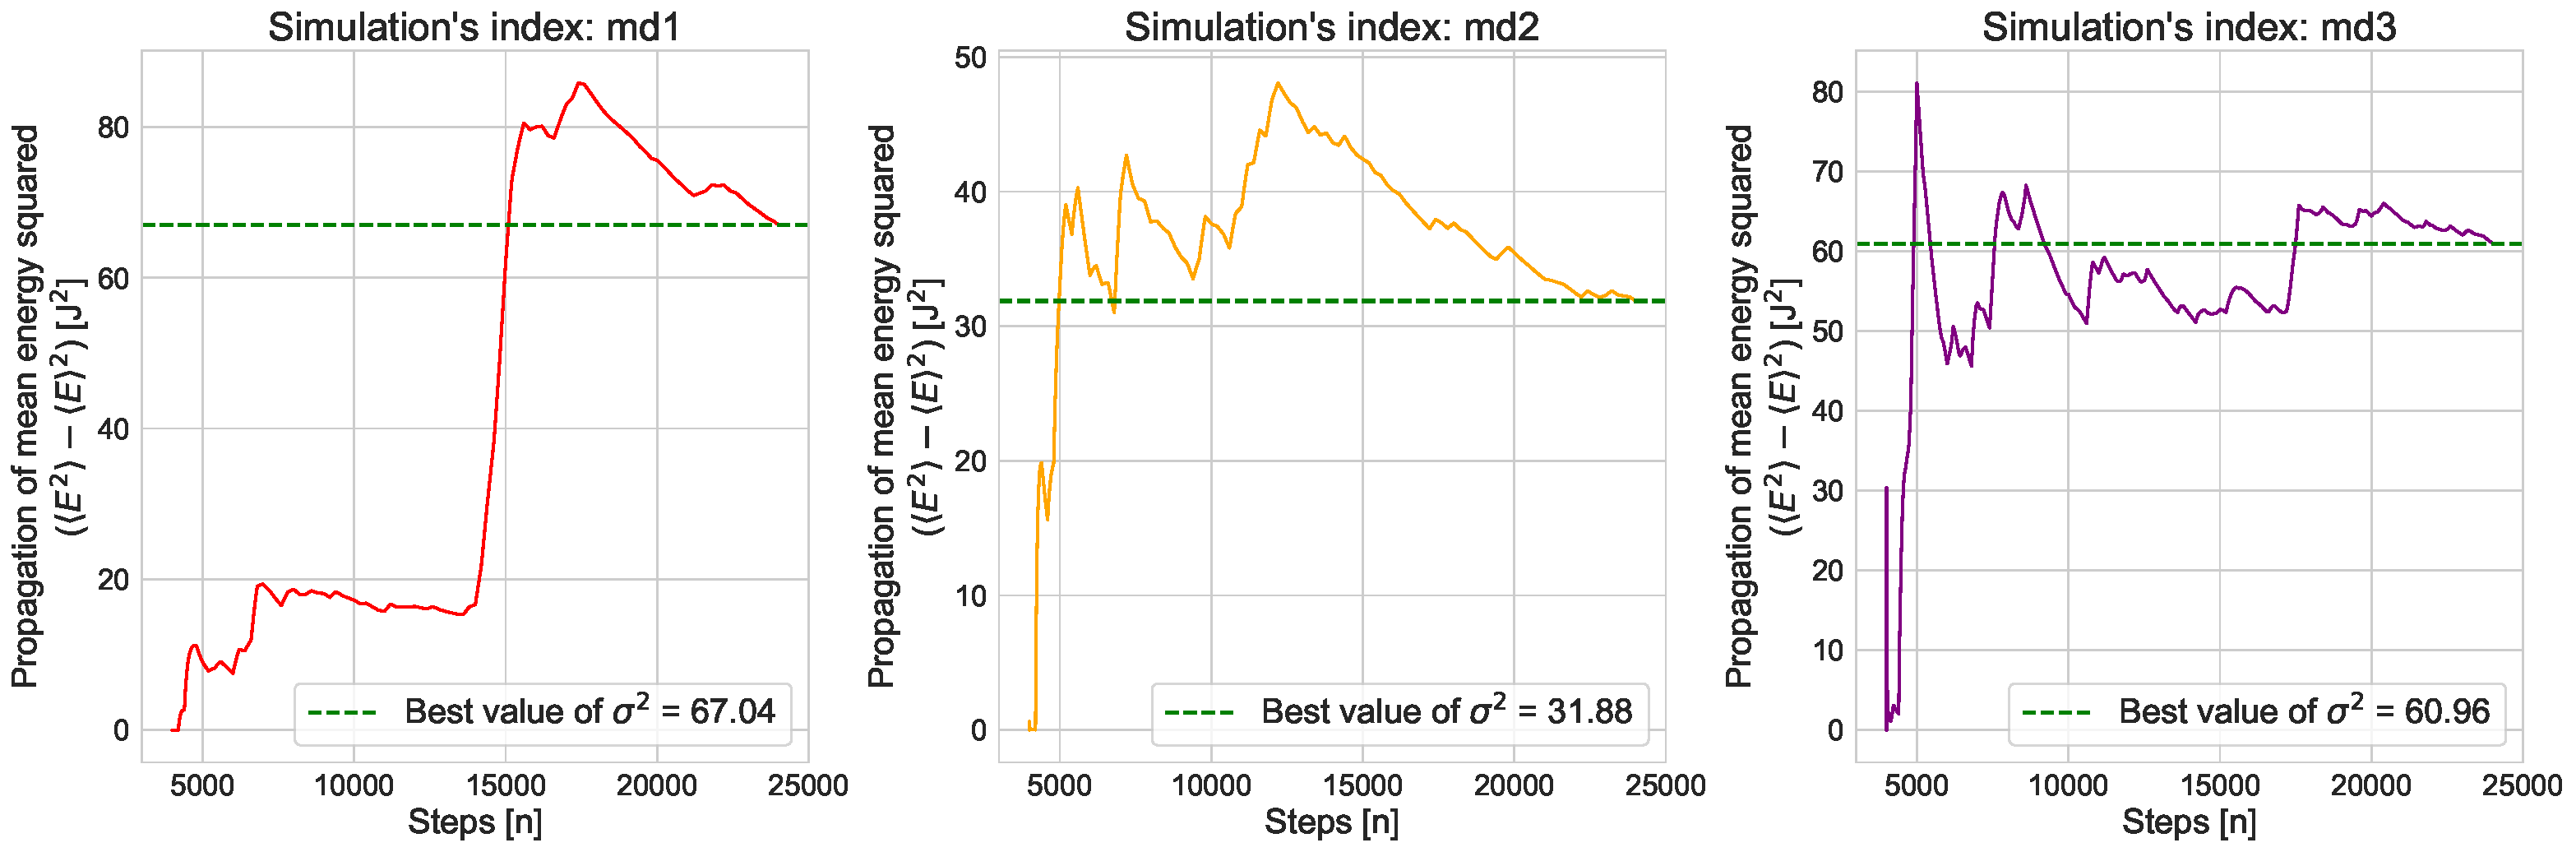
\includegraphics[width=\textwidth]{images/energy_oscill_24.pdf}}
\captionof{figure}{Az energia fluktuációja egyensúlyi állapotban ($\left< E^{2} \right> - \left< E \right>^{2}$) $N = 64$ részecske esetén} \label{fig:21}
\hfill \break \break
{\centering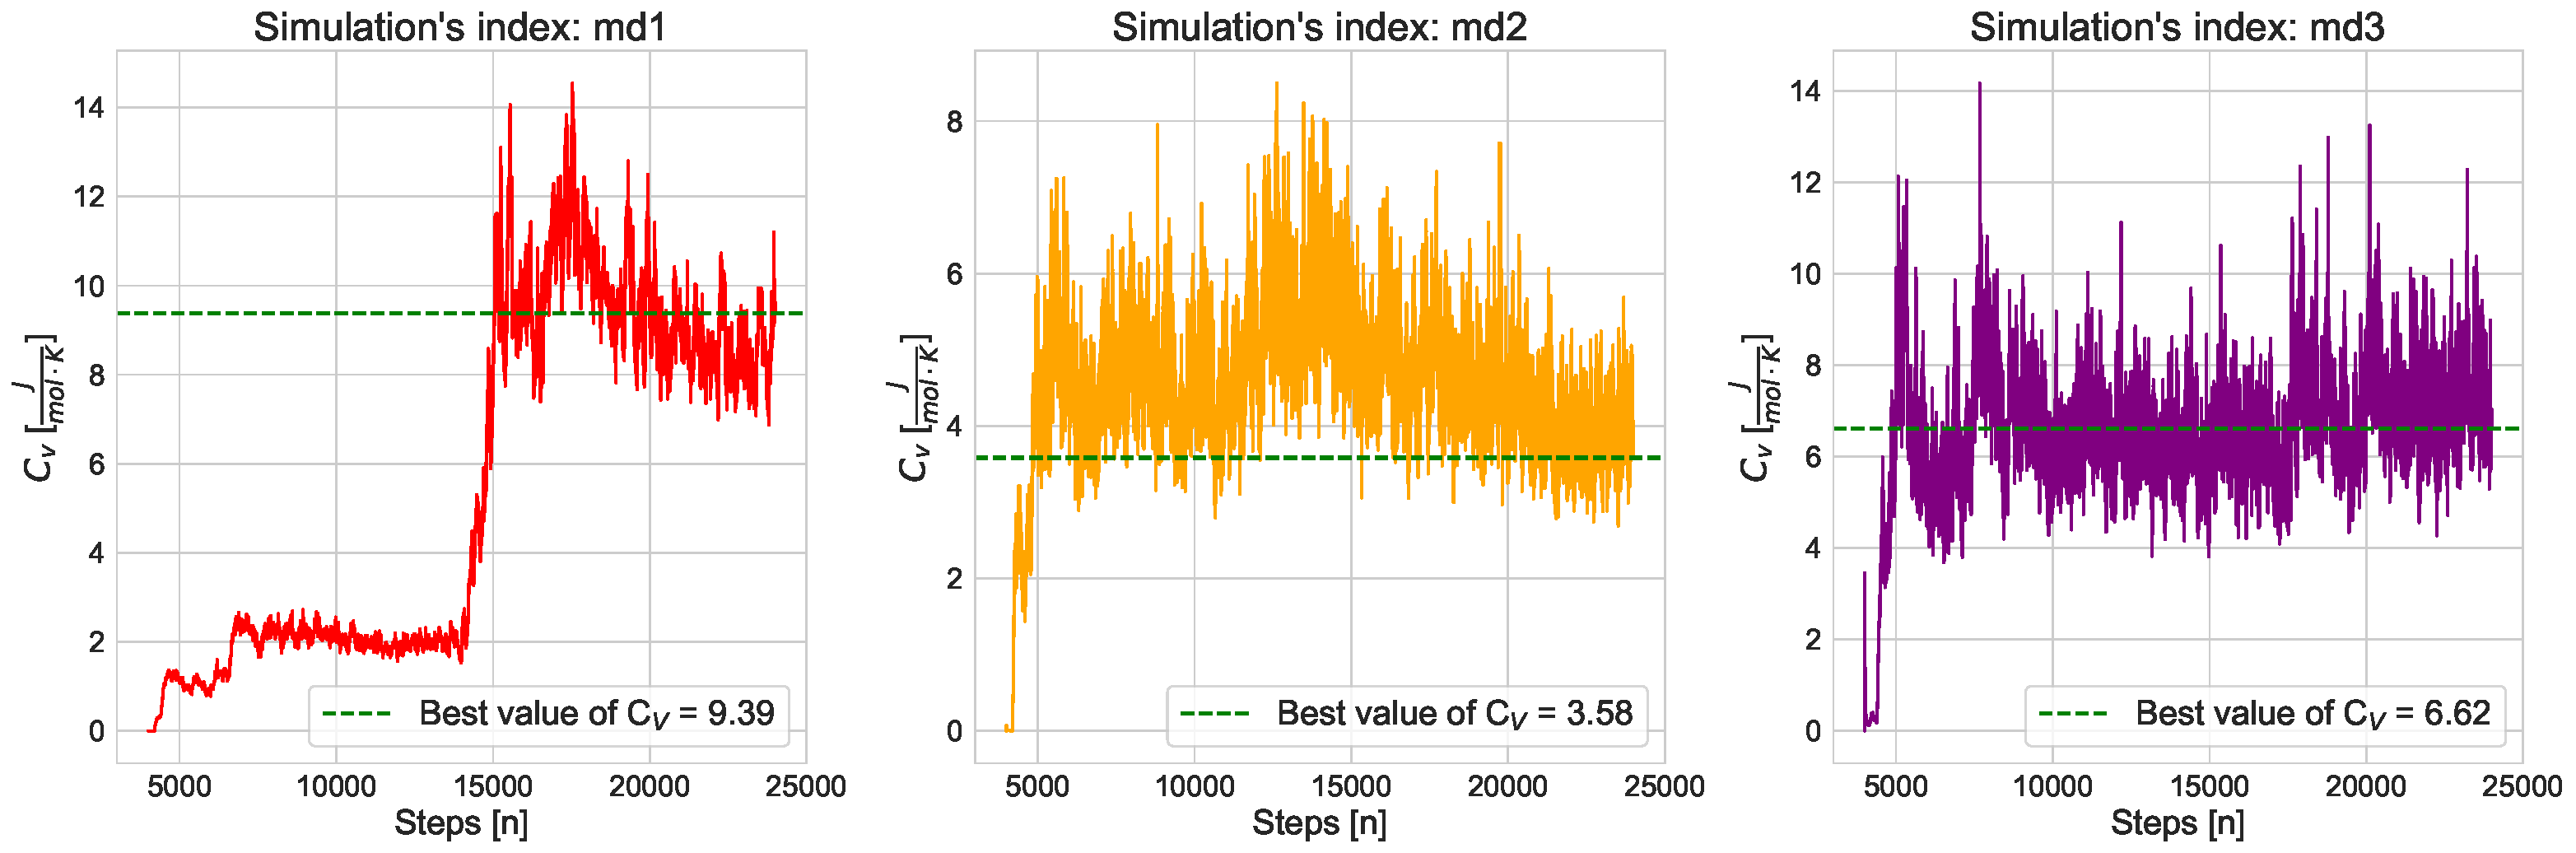
\includegraphics[width=\textwidth]{images/heat_capacity_propag_24.pdf}}
\captionof{figure}{A hőkapacitás közelítése egyensúlyi helyzetben $N = 64$ részecske esetén} \label{fig:22}
\hfill \break \break
{\centering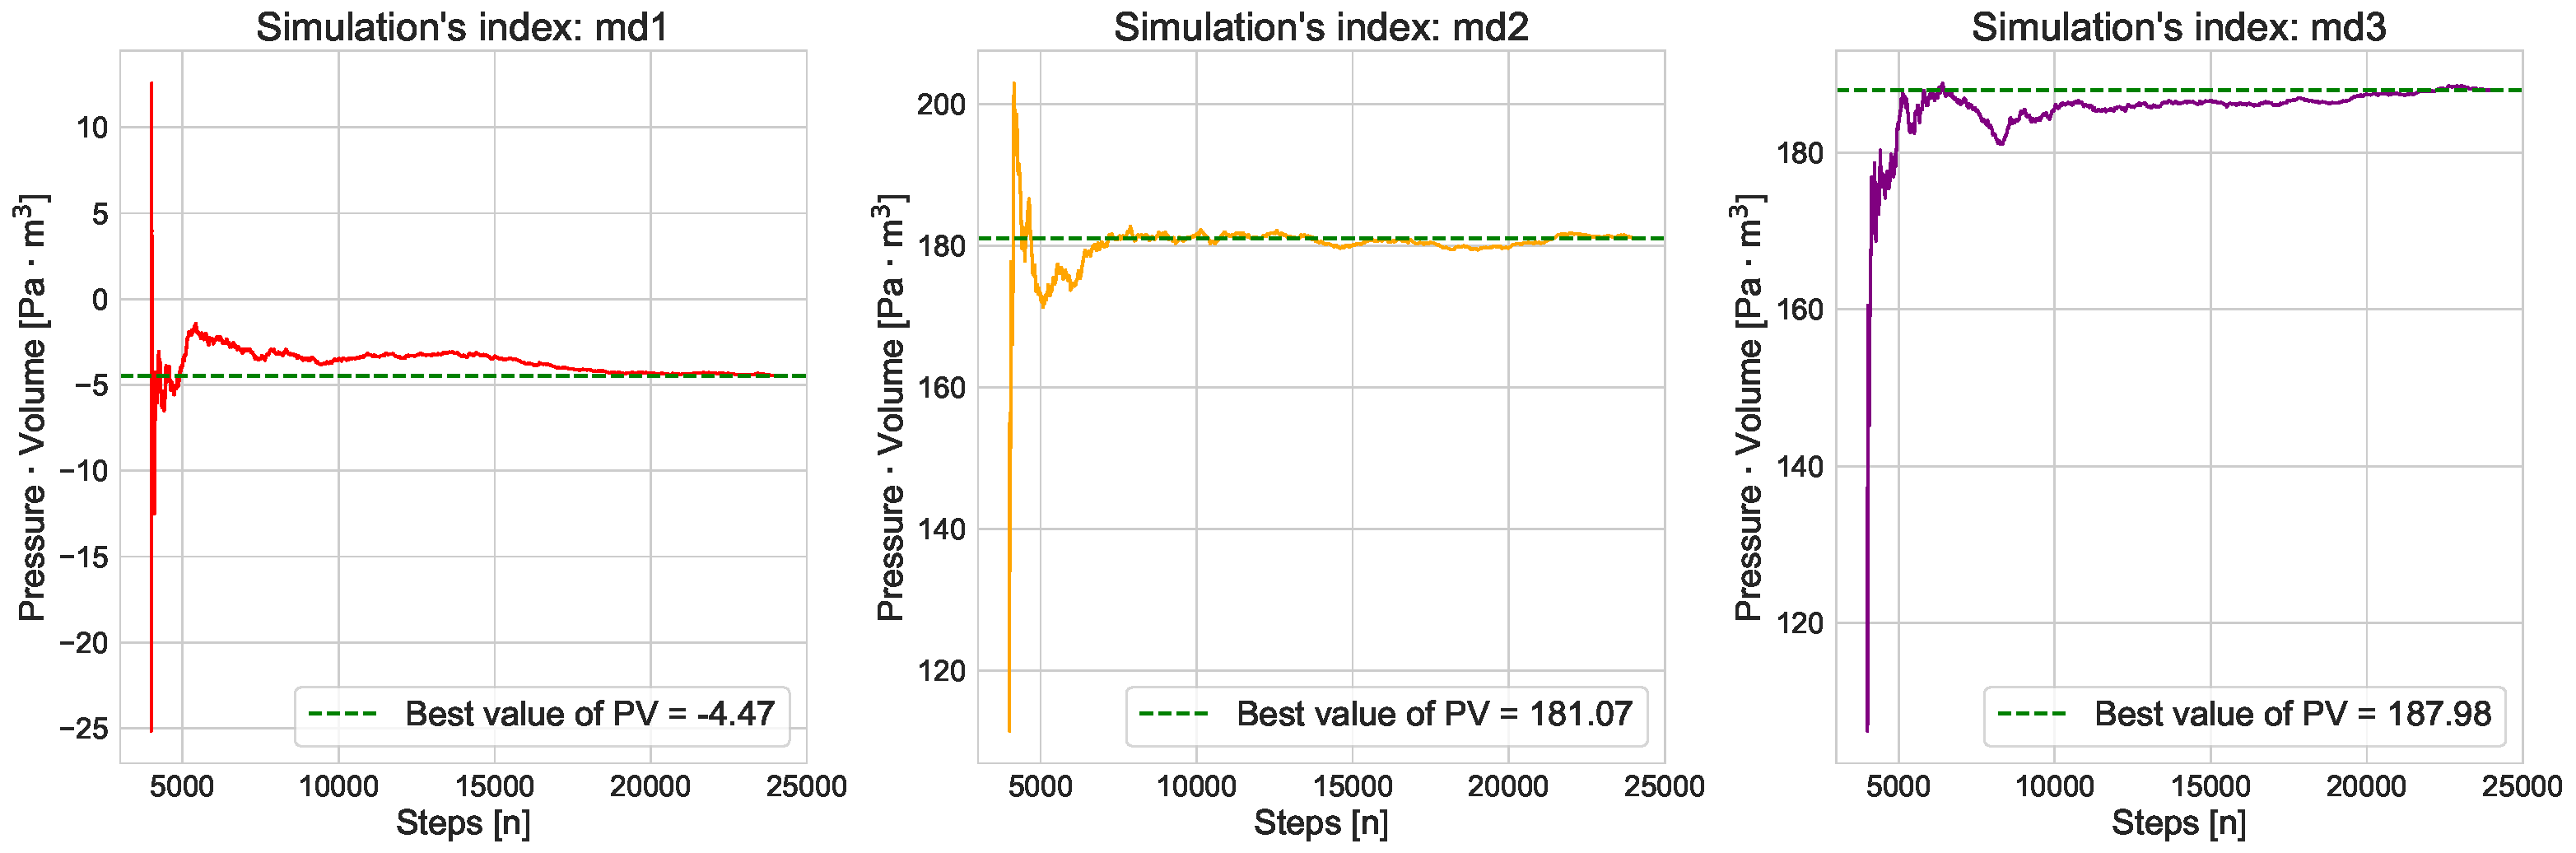
\includegraphics[width=\textwidth]{images/PV_24.pdf}}
\captionof{figure}{A $PV$ nyomás $\times$ térfogat érték ábrázolása, $N = 64$ részecske esetén} \label{fig:23}
\hfill \break \break
{\centering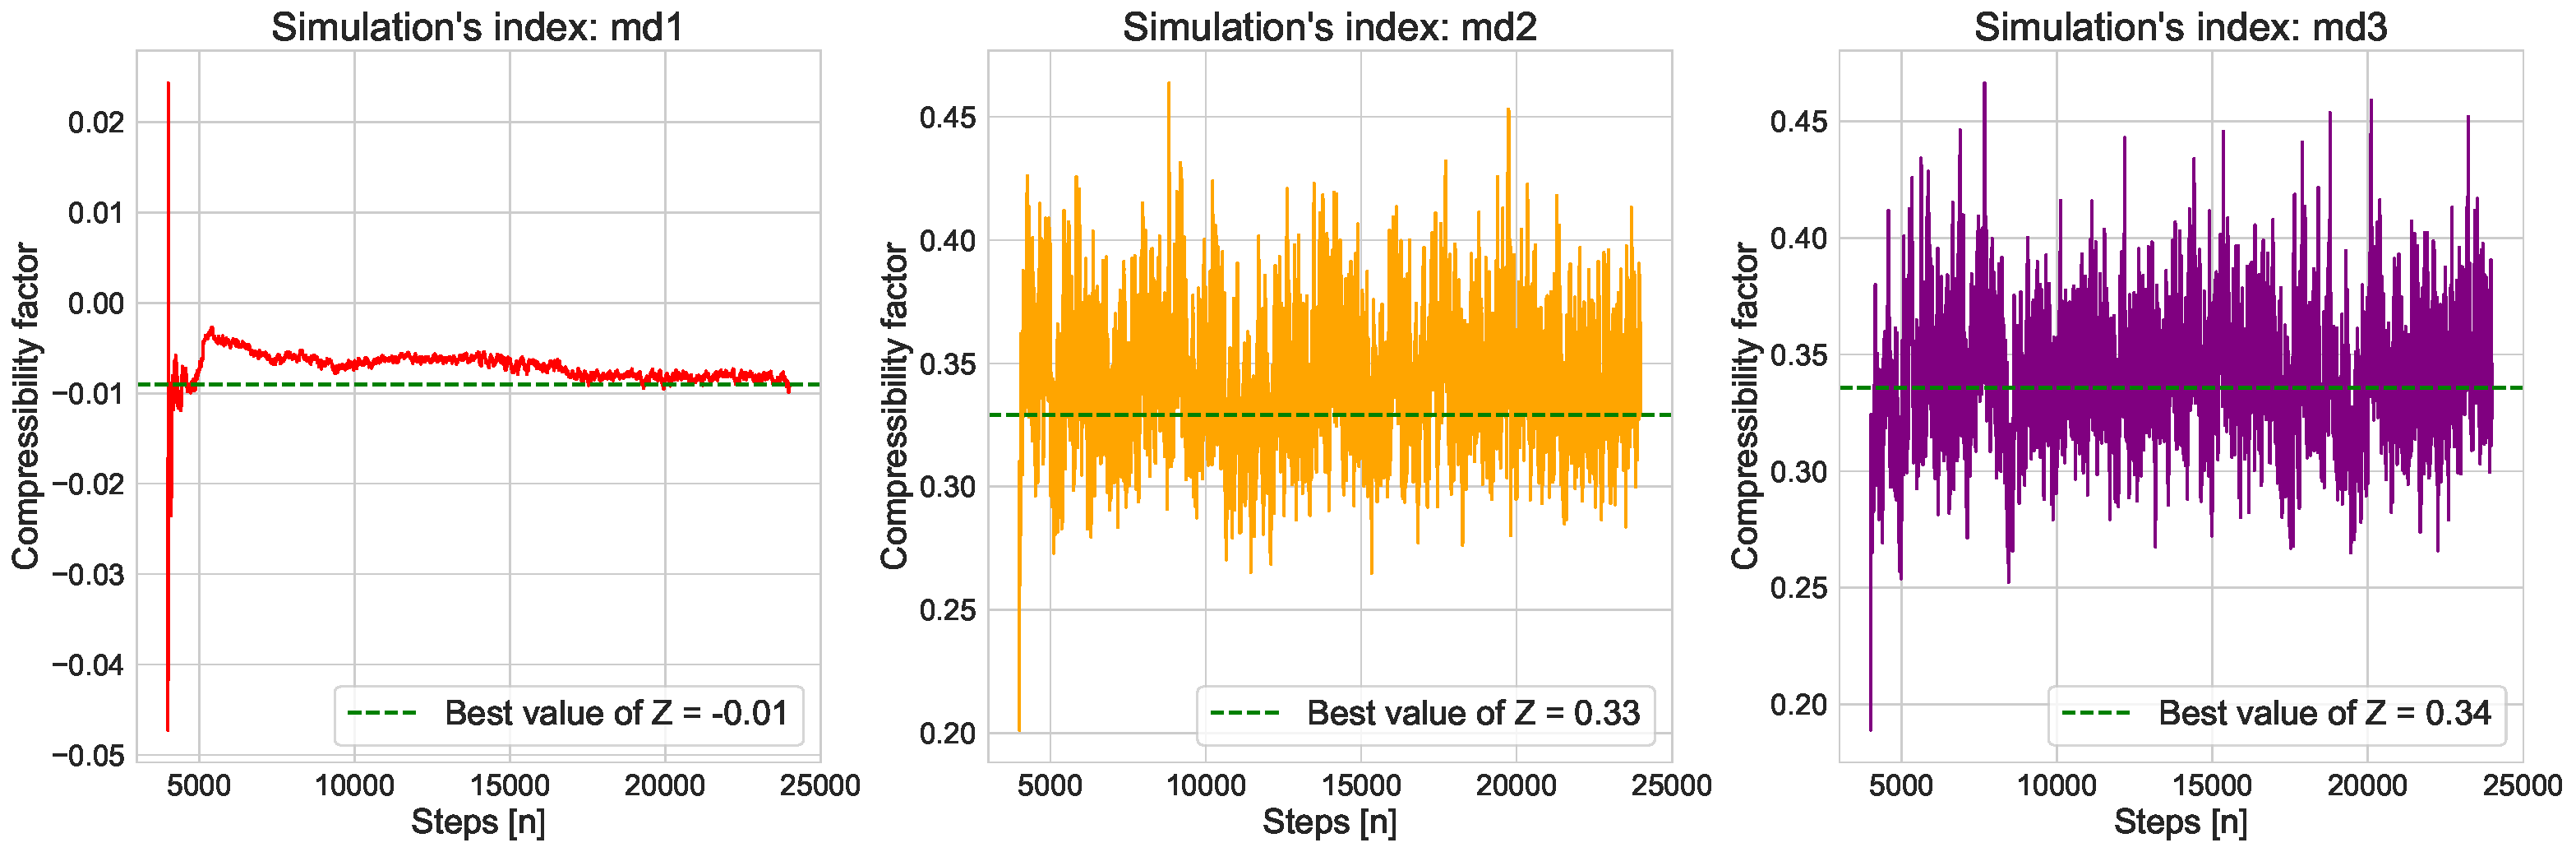
\includegraphics[width=\textwidth]{images/Z_24.pdf}}
\captionof{figure}{A kompresszibilitási faktor közelítése $N = 64$ részecske esetén} \label{fig:24}

\newpage

\subsection*{A.1.3\ \ Futásidők}

{\centering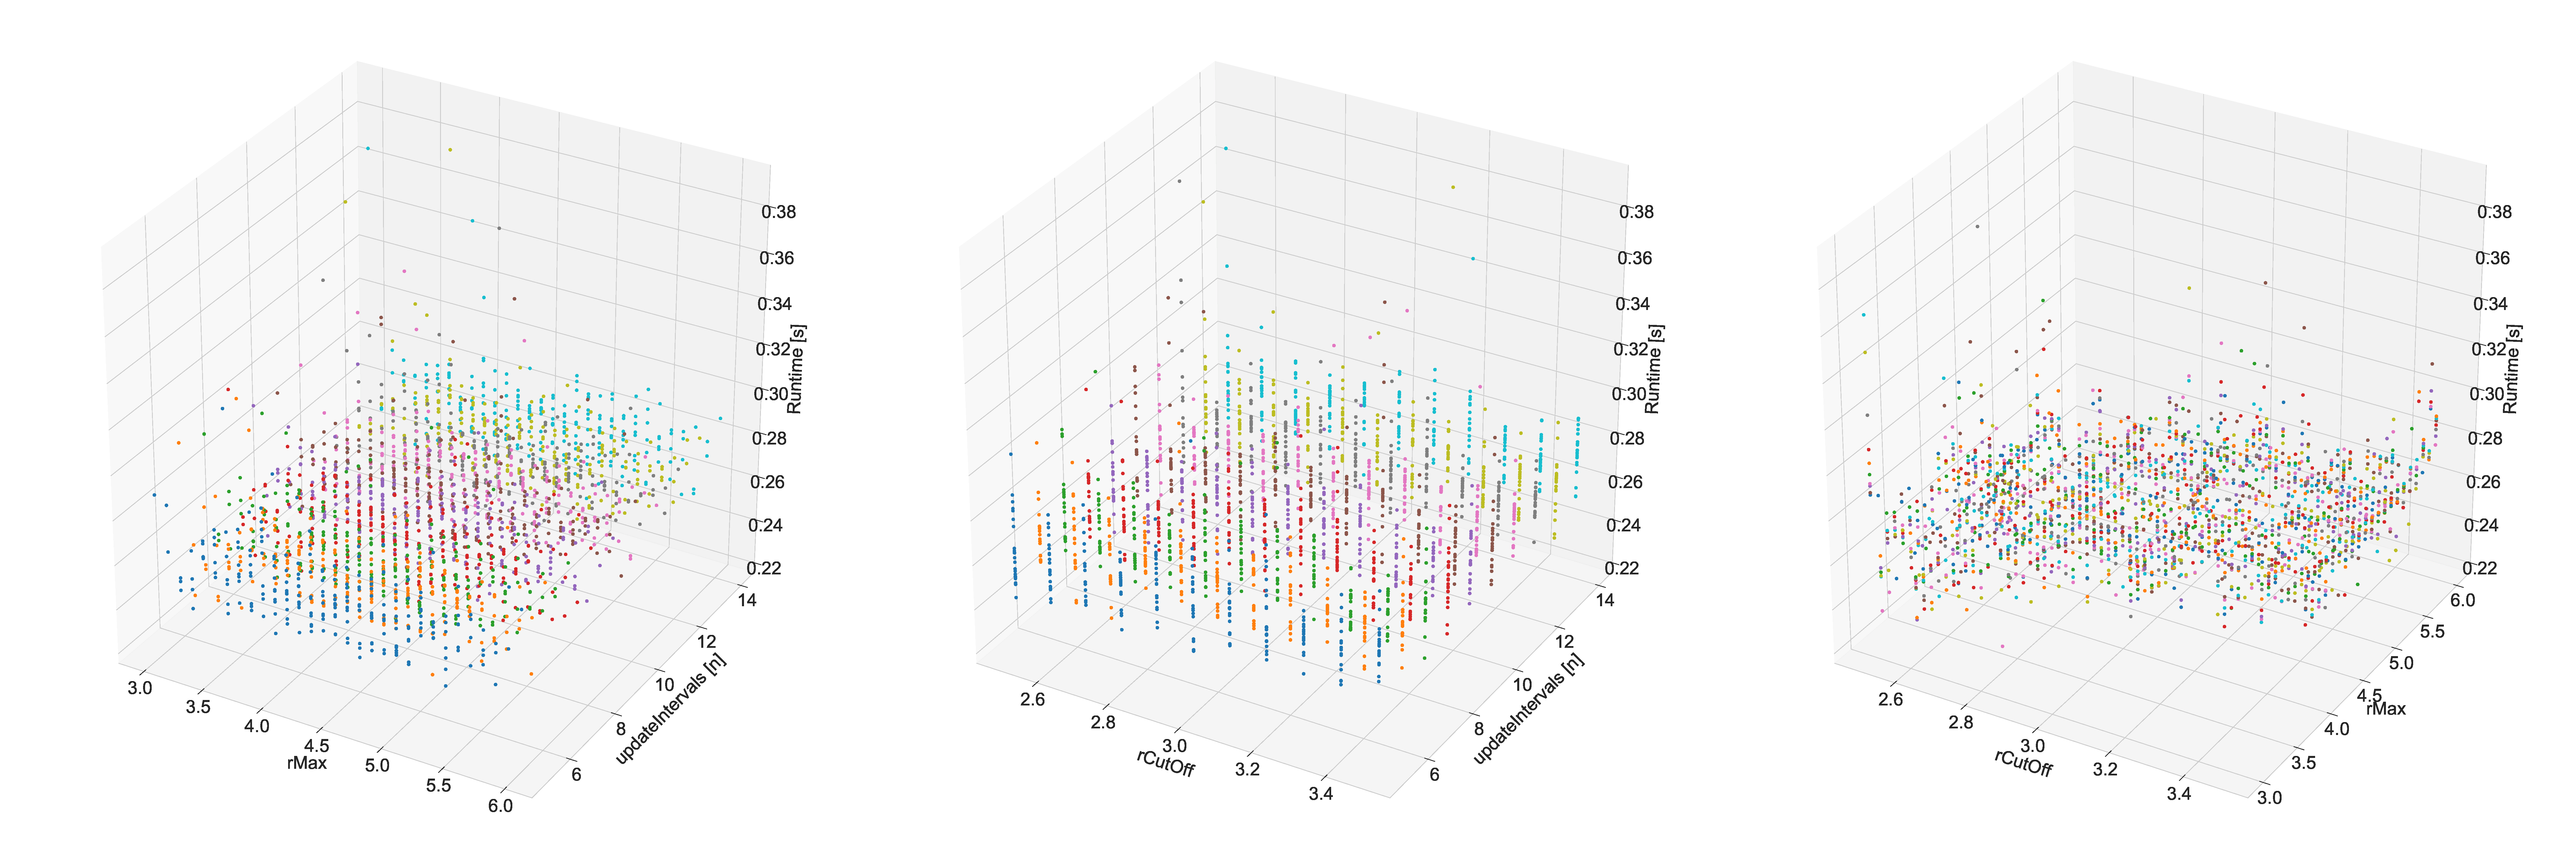
\includegraphics[width=\textwidth]{images/runtime_full_md3.pdf}}
\captionof{figure}{A futásidők teljes 4D terének 3D projekciói. Az azonos szimulációk mindhárom képen azonos színekkel vannak jelölve.\\Bal szélső ábra: Az egyes szimulációk futásideje az \texttt{rMax} és az \texttt{updateInterval} függvényében\\Középső ábra: A futásidők az \texttt{rCutOff} és \texttt{updateInterval} függvényében\\Jobb szélső ábra: A futásidők az \texttt{rCutOff} és \texttt{rMax} függvényében} \label{fig:23}

\hfill \break \break

{\centering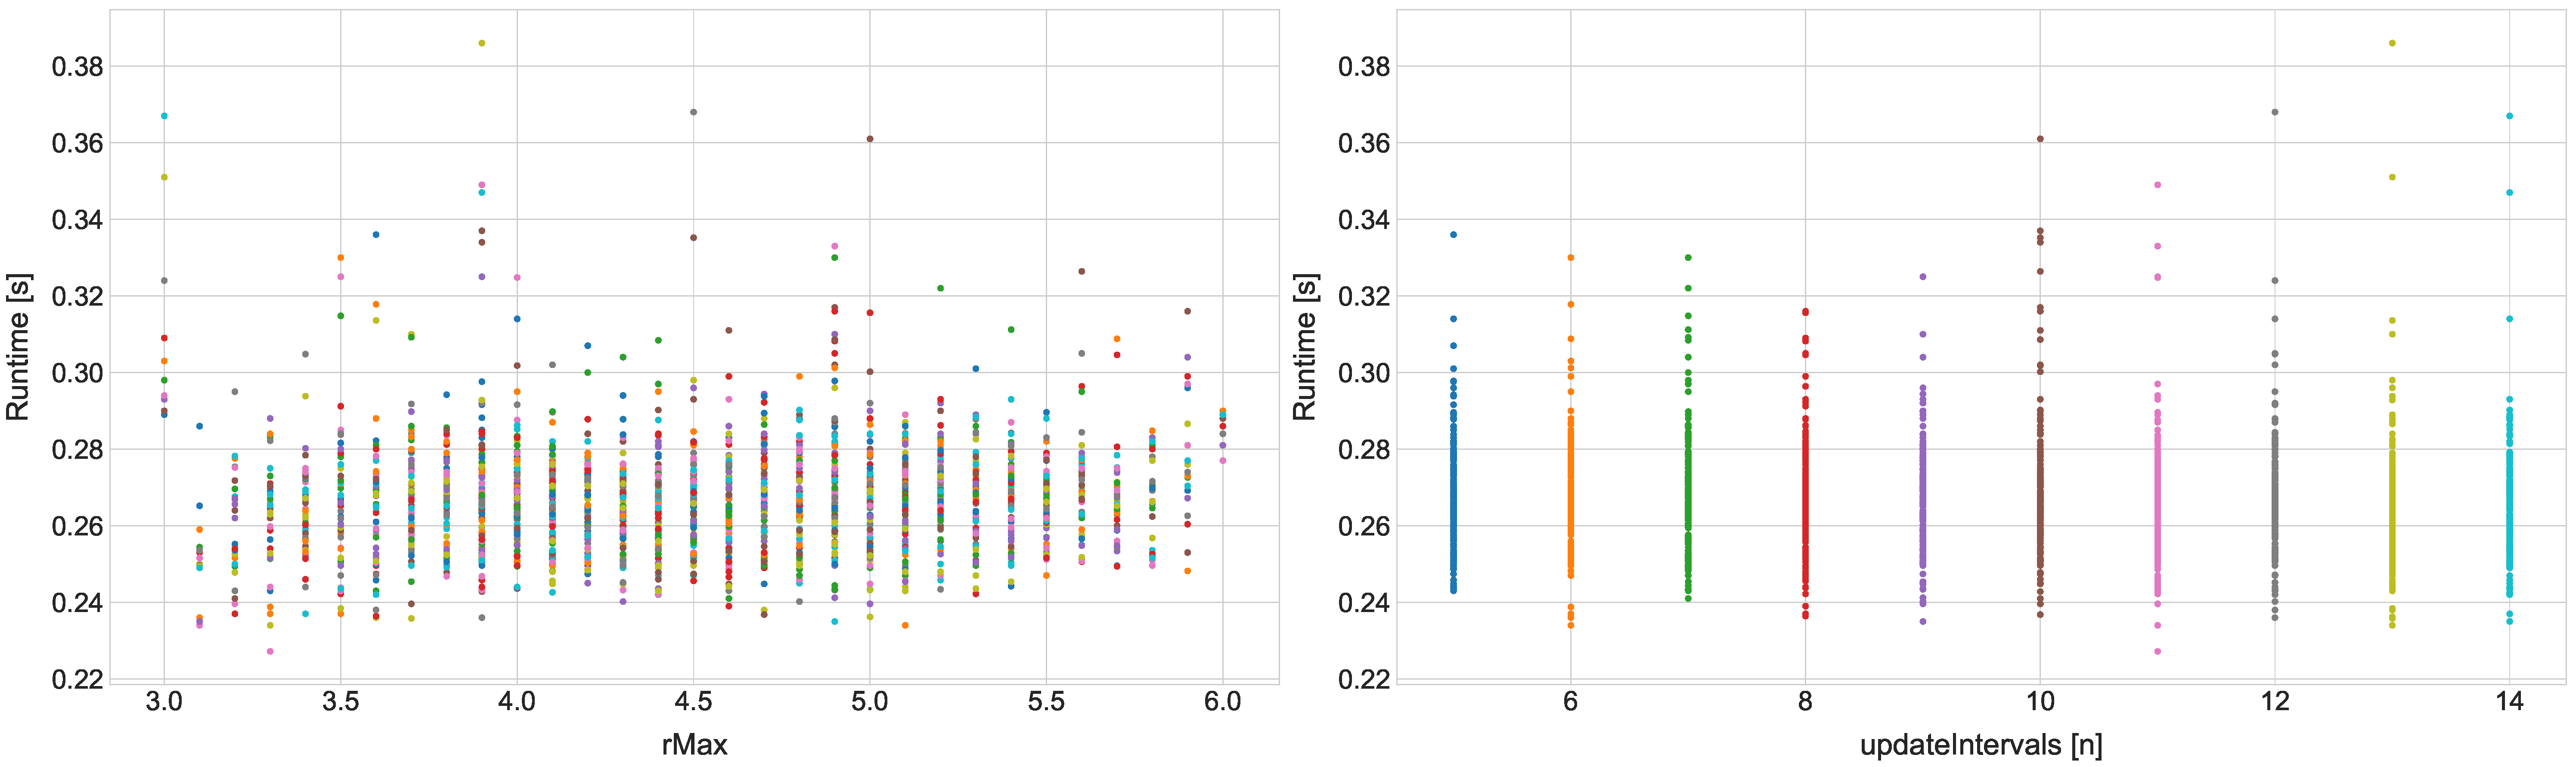
\includegraphics[width=\textwidth]{images/runtime_rmax_update_md3.pdf}}
\captionof{figure}{A futásidők első további 2D projekciói. Itt azok az \texttt{rMax} és \texttt{updateInterval} paraméterek függvényében vannak ábrázolva.} \label{fig:24}
\hfill \break \break
{\centering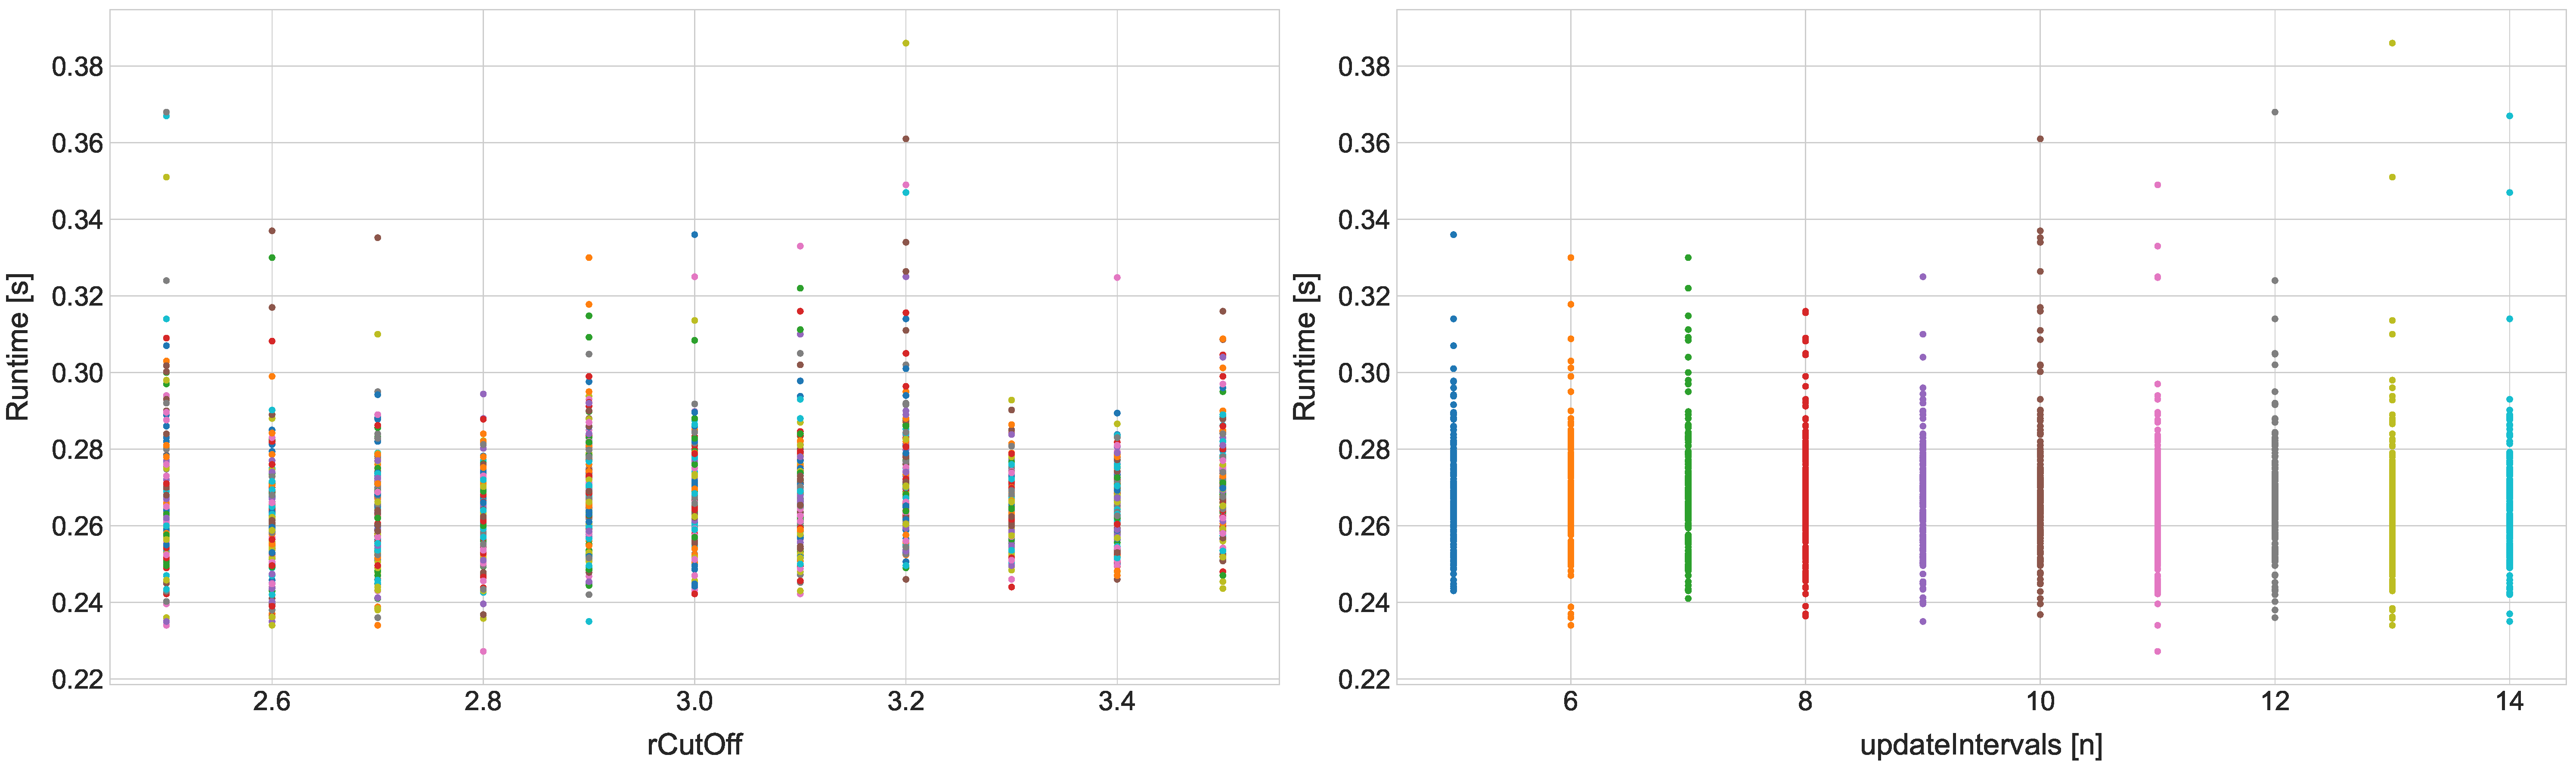
\includegraphics[width=\textwidth]{images/runtime_rcutoff_update_md3.pdf}}
\captionof{figure}{A futásidők második további 2D projekciói. Itt azok az \texttt{rCutOff} és \texttt{updateInterval} paraméterek függvényében vannak ábrázolva.} \label{fig:25}
\hfill \break \break
{\centering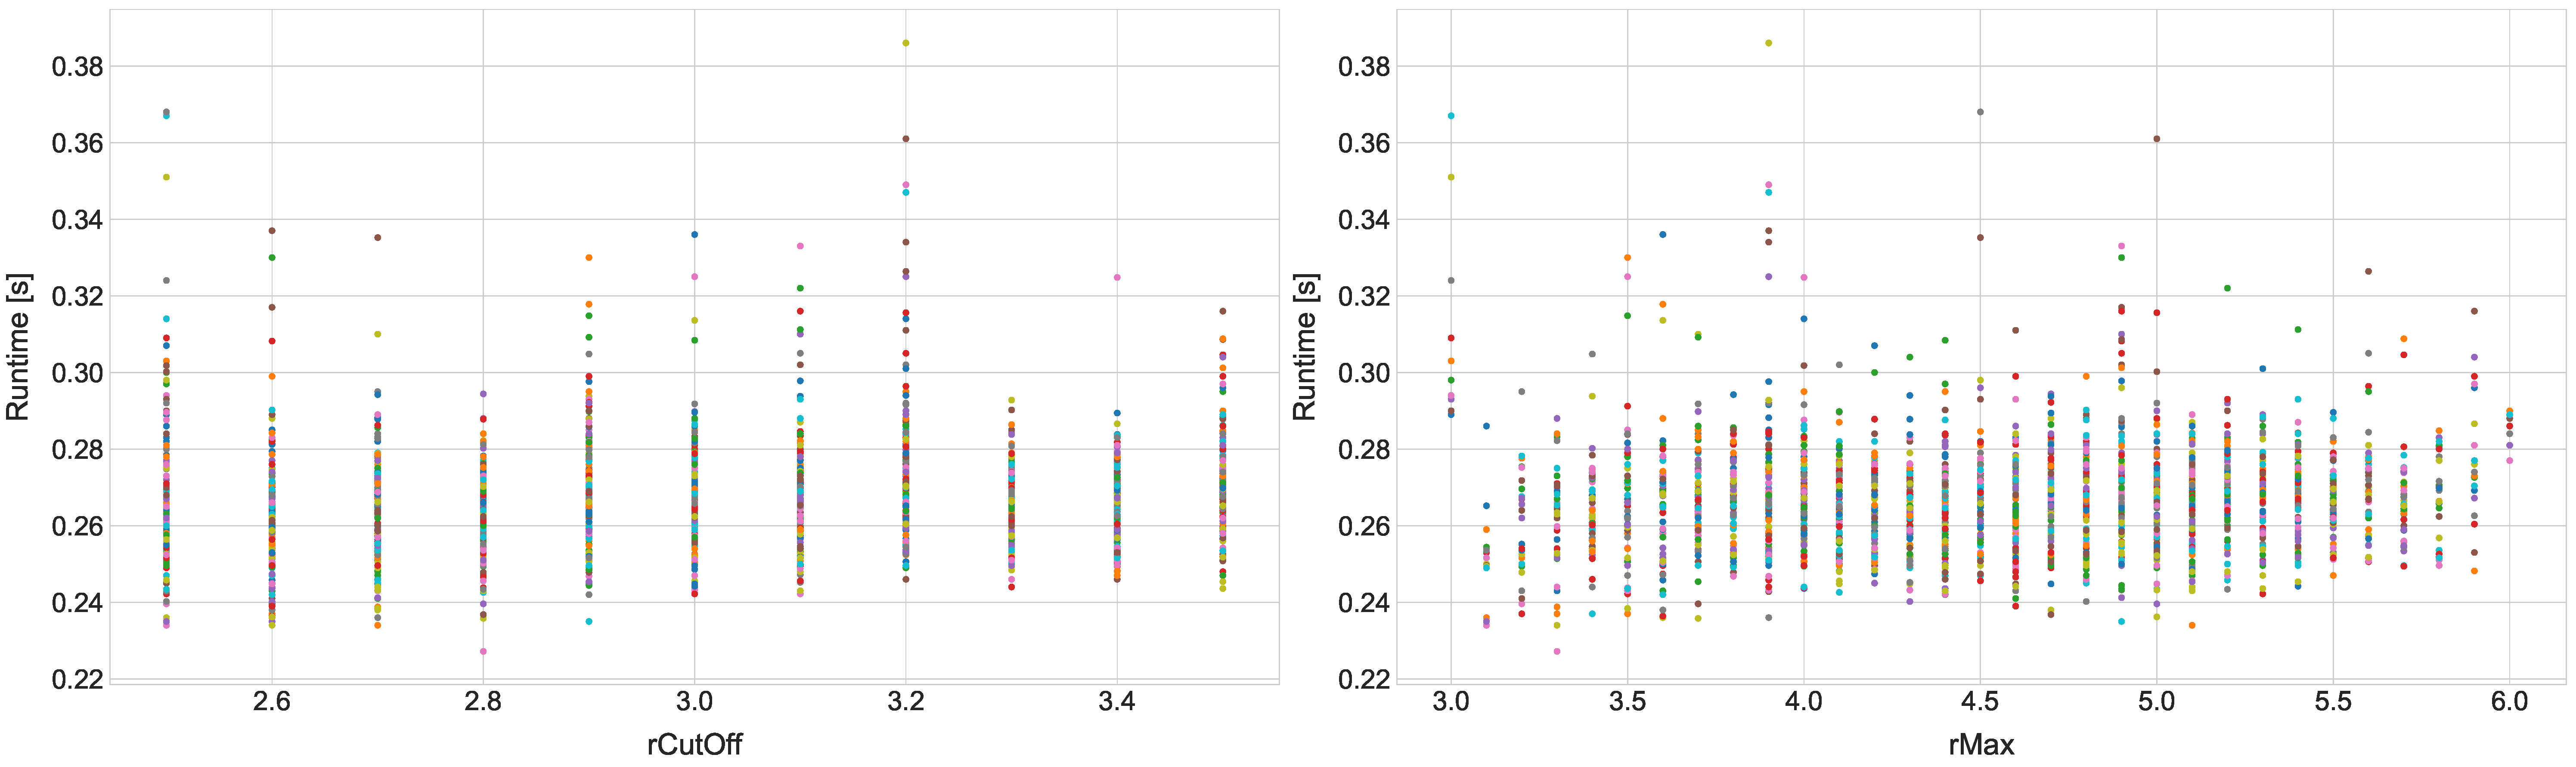
\includegraphics[width=\textwidth]{images/runtime_rcutoff_rmax_md3.pdf}}
\captionof{figure}{A futásidők harmadik további 2D projekciói. Itt azok az \texttt{rCutOff} és \texttt{rMax} paraméterek függvényében vannak ábrázolva.} \label{fig:26}